%!TEX root = ../thesis.tex
%*******************************************************************************
%****************************** Second Chapter *********************************
%*******************************************************************************

\chapter{Linear mixed models for eQTL mapping}
\label{chapter2}

In \textbf{Chapters 
% 3-6
\ref{chapter3}-\ref{chapter5}}
I describe 
% and develop
various models for \glspl{eqtl} mapping using single cell expression profiles. 
All of these models build on a 
linear mixed model (LMM)
% \gls{lmm}
framework. 
I use this chapter to provide an overview of linear and linear mixed models and their application in quantitative genetics, with a focus on their use for \gls{eqtl} mapping. 
I will also briefly introduce \gls{lmm}-based models to test for \gls{gxe} interactions, to provide the necessary theoretical foundations for some of the analyses in \textbf{Chapter 
% 4
\ref{chapter4}}.
% and \textbf{
% 6
% \ref{chapter6}}.
\\

\gls{lmm}s are a very popular framework for many genetic analyses. 
They are especially appealing because they provide robust control for confounding factors. 
One drawback of these methods is that inference using \gls{lmm}s is typically computationally costly, yet efficient implementations of specific \gls{lmm}s exist, enabling application to large cohorts. 
I use this chapter to provide an overview of the use of \gls{lmm}s in genetic association studies: in \textbf{sections \ref{sec:linear_regression}-\ref{sec:linear_models_genetics}}, I discuss the linear model (also called linear regression) and basic applications for genome-wide association studies (GWAS) and \gls{qtl} mapping. 
In \textbf{section \ref{sec:linear_mixed_models}}, I introduce the \gls{lmm} and discuss applications in genetics, with a focus on the use of \gls{lmm}s for \gls{eqtl} mapping. 
Finally, in \textbf{section \ref{sec:lmm_gxe}}, I briefly discuss extensions of the \gls{lmm} framework to test for \gls{gxe} interactions.\\

\newpage

For mathematical model descriptions throughout this thesis, I use the following notation: bold, lower-case letters symbolise one-dimensional column vectors (e.g. $\mathbf{v}$) and bold capitalised letters matrices (e.g. $\mathbf{M}$). 
A normal distribution is specified by $ \mathcal{N}(\mu, \sigma^2)$, where $\mu$, $\sigma$ are two scalars representing the mean and standard deviation parameters.
For simplicity, I use the same notation for multivariate normal (e.g. $ \mathcal{N}(\boldsymbol{\mu}, \boldsymbol{\Sigma})$), noting that the specified parameters ($\boldsymbol{\mu}$ and $\boldsymbol{\Sigma}$) are an $N \times 1$ mean vector, and an $N \times N$ covariance matrix, respectively.

%********************************** %First Section  **************************************

\section{The linear regression model} 
\label{sec:linear_regression}

A linear model, or regression, is a statistical approach to modelling a continuous output variable (dependent variable, or outcome) as a linear function of one or more input variables (features, or independent variables). 
For $F$ features, the outcome variable for a single sample $i$ can be specified as:

\begin{equation} \label{eq:Linear_regression_sample_i}
 y_i = \sum_{f=1}^{F} x_{i,f}\beta_f + \psi_i,
\end{equation}

where the noise term $\psi_i$ ($ \psi_i \sim \mathcal{N}(0, \sigma_n^2)$) accounts for measurement noise of $y_i$, reflecting the non-deterministic relationship between $y_i$ and $x_{i,f}$, and is assumed to follow a normal distribution with $0$ mean and constant variance $\sigma_n^2$. 
Furthermore, the noise term is assumed to be independent across samples, i.e. $cov(\psi_i, \psi_j)=0$ for every $i \neq j$. 
For $N$ samples, the model in eq. \eqref{eq:Linear_regression_sample_i} can be expressed in matrix form as:

\begin{equation} \label{eq:Linear_regression_matrix_form}
\mathbf{y} = \mathbf{X}\boldsymbol{\beta} + \boldsymbol{\psi}, 
\end{equation}

where $\mathbf{y}$ is the $N \times 1$ outcome vector, $\mathbf{X}$ is the $N \times F$ feature matrix, and $\boldsymbol{\beta}$ is the $F \times 1$ corresponding weight vector. 
Finally, $\boldsymbol{\psi}$ is the $N \times 1$ noise vector such that: $\boldsymbol{\psi}\sim \mathcal{N}(\mathbf{0}, \sigma_n^2 \mathbf{I_N})$, where $\mathbf{I_N}$ denotes the $N \times N$ identity matrix. 

% \newpage

\subsection{The maximum likelihood solution}

Equation \eqref{eq:Linear_regression_matrix_form} is a realisation of the probability distribution of the data $p(\mathbf{y}| \mathbf{X}, \boldsymbol{\beta}, \sigma_n^2)$ given the input variables $\mathbf{X}$ and the model parameters $\boldsymbol{\beta}$ and $\sigma_n^2$.
This is known as the likelihood of the model and is considered as a function of the model parameters, denoted as $\mathcal{L}(\boldsymbol{\beta}, \sigma_n^2)$. 
We can then express the model in eq. \eqref{eq:Linear_regression_matrix_form} as:

\begin{equation} \label{eq:Linear_regression_likelihood}
 \mathcal{L}(\boldsymbol{\beta}, \sigma_n^2) = p(\mathbf{y}| \mathbf{X}, \boldsymbol{\beta}, \sigma_n^2) = \mathcal{N}(\mathbf{y} | \mathbf{X}\boldsymbol{\beta}, \sigma_n^2 \mathbf{I_N}),
\end{equation}

\newpage

or, 
equivalently,
% more explicitly, 
as:

\begin{equation} \label{eq:Linear_regression_MVN_form}
\mathbf{y} \sim \mathcal{N}(\mathbf{X}\boldsymbol{\beta}, \sigma_n^2 \mathbf{I_N}). 
\end{equation}

In parameter inference, the maximum likelihood estimator (MLE) of the model parameters is defined as the set of parameter values that maximise the likelihood.
% Intuitively, this selects the parameter values that make the observed data most probable.
In practice, it is often convenient to work with the natural logarithm of the likelihood function, called the log likelihood ($\ell = \log \mathcal{L}$), noting that both functions will be maximised by the same parameter values.
The log likelihood of the model can be explicitly specified as:\\

\begin{equation} \label{eq:Linear_regression_log_likelihood}
\begin{split}
 \ell(\boldsymbol{\beta}, \sigma_n^2) = -\frac{1}{2} \bigg\{N \log (2\pi\sigma_n^2) + \log |\mathbf{I_N}|+ \frac{1}{\sigma_n^2}(\mathbf{y}-\mathbf{X}\boldsymbol{\beta})^T\mathbf{I_N}^{-1}(\mathbf{y}-\mathbf{X}\boldsymbol{\beta}) \bigg\} \\
= -\frac{N}{2} \log (2\pi) - \frac{N}{2} \log(\sigma_n^2)- 0 - \frac{1}{2\sigma_n^2}(\mathbf{y}-\mathbf{X}\boldsymbol{\beta})^T(\mathbf{y}-\mathbf{X}\boldsymbol{\beta}). 
\end{split}
\end{equation}

Denoting with $\hat{\boldsymbol{\beta}}$ and $\hat{\sigma_n^2}$ the \gls{mle}s of $\boldsymbol{\beta}$ and $\sigma_n^2$, we can write:

\begin{equation} \label{eq:Linear_regression_MLEs}
\hat{\boldsymbol{\beta}},\hat{\sigma_n^2} = \mathrm{argmax}_{\boldsymbol{\beta},\sigma_n^2} \ \ell(\boldsymbol{\beta}, \sigma_n^2). 
\end{equation} 

By setting the gradient of the log likelihood in eq. \eqref{eq:Linear_regression_log_likelihood} with respect to both parameters to zero, and solving the joint system:

\begin{equation} \label{eq:Linear_regression_MLE_system}
\systeme{
    \dfrac{\partial \ell(\boldsymbol{\beta}, \sigma_n^2)}{\partial \boldsymbol{\beta}} = \mathbf{0},
    \dfrac{\partial \ell(\boldsymbol{\beta}, \sigma_n^2)}{\partial \sigma_n^2} = 0
    },
\end{equation}

We find:

\begin{equation} \label{eq:Linear_regression_MLE_solution_beta}
\hat{\boldsymbol{\beta}} = (\mathbf{X}^T\mathbf{X})^{-1}\mathbf{X}^T\mathbf{y} 
\end{equation}

and

\begin{equation} \label{eq:Linear_regression_MLE_solution_sigma}
 \hat{\sigma_n^2} = \frac{1}{N}(\mathbf{y}-\mathbf{X}\hat{\boldsymbol{\beta}})^T(\mathbf{y}-\mathbf{X}\hat{\boldsymbol{\beta}}) = \frac{1}{N}(\mathbf{y}-\mathbf{X}(\mathbf{X}^T\mathbf{X})^{-1}\mathbf{X}^T\mathbf{y})^T(\mathbf{y}-\mathbf{X}(\mathbf{X}^T\mathbf{X})^{-1}\mathbf{X}^T\mathbf{y}). 
\end{equation}

Note that the solution for $\hat{\boldsymbol{\beta}}$ in eq. \eqref{eq:Linear_regression_MLE_solution_beta} is equivalent to the \gls{ols} solution \cite{hayashi2000econometrics}.

\newpage

\subsection{The restricted maximum likelihood solution}

% OS: add maybe a line or two of motivation *why* we are interested in a reml estimate??

In Gaussian models as in eq. \eqref{eq:Linear_regression_MVN_form} the \gls{mle} of the variance parameter $\hat{\sigma_n^2}$ suffers from downward bias\footnote{The bias of an estimator refers to the difference between this estimator’s expectation (here, $E[\hat{\sigma_n^2}]$) and the true parameter value ($\sigma_n^2$).
Downward bias indicates that $E[\hat{\sigma_n^2}] < \sigma_n^2$.} because the weights $\hat{\boldsymbol{\beta}}$ are estimated from the data, which involves a reduction of the effective number of degrees of freedom. \\

Patterson and Thompson \cite{patterson1971recovery} presented a $\boldsymbol{\beta}$-free estimation of $\sigma_n^2$ via the restricted (or residual) maximum likelihood (ReML).
Given the model in eq. \eqref{eq:Linear_regression_matrix_form} the ReML can be obtained by projecting the output vector in a space that is orthogonal to $\mathbf{X}$ such that:

\begin{equation}\label{eq:REML_0_projection}
    \mathbf{A}\mathbf{X} = \mathbf{0}.
\end{equation}

Using eq. \eqref{eq:REML_0_projection} and rewriting eq. \eqref{eq:Linear_regression_matrix_form} in terms of the projection $\mathbf{w}$ we obtain:

\begin{equation}\label{eq:REML_w_projection}
    \mathbf{w} = \mathbf{A}\mathbf{y} = \mathbf{A}(\mathbf{X}\boldsymbol{\beta} + \boldsymbol{\psi}) = \mathbf{A}\boldsymbol{\psi},
\end{equation}

which provides an expression of $\mathbf{y}$ that is independent of $\boldsymbol{\beta}$.\\

By estimating $\ell(\sigma_n^2 | \mathbf{A}\mathbf{y})$ for the model in eq. \eqref{eq:Linear_regression_MVN_form}, we derive the log restricted maximum likelihood:

\begin{equation} \label{eq:Linear_regression_log_restricted_likelihood}
\begin{split}
\ell(\sigma_n^2) = -\frac{N-F}{2}\log (2\pi\sigma_n^2) - \frac{1}{2}\log |\mathbf{X}^T\mathbf{X}| 
- \frac{1}{2\sigma_n^2}(\mathbf{y}-\mathbf{X}\hat{\boldsymbol{\beta}})^T(\mathbf{y}-\mathbf{X}\hat{\boldsymbol{\beta}})  
\end{split},
\end{equation}

which is maximised by:

\begin{equation}\label{eq:Linear_regression_REML_sigma}
\hat{\sigma_n^2}_{ReML} =  \frac{1}{N-F}(\mathbf{y}-\mathbf{X}(\mathbf{X}^T\mathbf{X})^{-1}\mathbf{X}^T\mathbf{y})^T(\mathbf{y}-\mathbf{X}(\mathbf{X}^T\mathbf{X})^{-1}\mathbf{X}^T\mathbf{y}),
\end{equation}

which is now an unbiased\footnote{i.e. $E[\hat{\sigma_n^2}_{ReML}] = \sigma_n^2$.} estimator for $\sigma_n^2$. \\

Note that eq. \eqref{eq:Linear_regression_REML_sigma} is identical to eq. \eqref{eq:Linear_regression_MLE_solution_sigma} except for the fact that $N$ is replaced by ($N-F$), denoting the loss of $F$ degrees of freedom.

\newpage

%********************************** %Second Section  **************************************

\section{Regression models for association studies}
\label{sec:linear_models_genetics}

As we have seen (\textbf{section \ref{sec:gwas}}), originally GWA studies used contingency table tests (such as the $\chi^2$ test) to assess the significant effect of a variant on a dichotomous trait \cite{mccarthy2008genome}.
However, these tests are sub-optimal in the case of quantitative traits, such as height and weight, which would need to be arbitrarily discretised.
Additionally, these tests are not equipped to account for confounding factors (these are described in more detail in \textbf{section \ref{sec:linear_mixed_models}}).
As a consequence, regression-based models became the preferred approach, because they allow covariate adjustment, and can directly provide a measure of the effect size for each tested variant \cite{bush2012genome}.\\

When applying regression models in genetic association studies, the phenotype of interest is modeled as the outcome variable ($\mathbf{y}$). 
In \gls{gwas}, we typically look at \textcolor{blue}{`organismal phenotypes'}, including traits such as height and eye colour or disease status/risk for complex disorders \cite{mccarthy2008genome}.
In (molecular) \gls{qtl} mapping, we consider `molecular phenotypes', such as gene expression (i.e. e\gls{qtl}), or protein level (p\gls{qtl}).
\\

The genotype at the \gls{snp} of interest is modelled as the independent variable.
We assume all \gls{snp}s to be biallelic, that is that they can only assume two possible values - A (major allele) and a (minor allele)\footnote{The notation of major and minor alleles refers to the allele frequency in the population studied.
Alternatively, it is possible to denote A as the reference allele and a as the alternative allele, based on the reference genome.}. 
Three models can be considered for the minor allele a.
First, a dominant model (i.e. AA = 0, Aa = 1, aa = 1; where one copy of the minor allele is sufficient to have a phenotypic effect); second, a recessive model, (AA = 0, Aa = 0, aa = 1; where two copies of the minor allele are necessary for observing a phenotypic effect); finally, an additive model (AA = 0, Aa = 1, aa = 2; where the phenotypic effect is proportional to the number of minor allele copies). 
Throughout this thesis, we will consider an additive genetic model, which is commonly used in both GWAS and eQTL mapping analyses \cite{laird2010fundamentals}.
\\

The test, then, consists of assessing the effect of each individual \gls{snp} ($\mathbf{g}$) on the phenotype ($\mathbf{y}$), one at a time.
For quantitative traits, including molecular traits such as gene expression and some complex traits such as height, blood pressure or BMI\footnote{BMI: body mass index, a measure of weight normalised by height.}, a linear regression is typically used\footnote{In contrast, case-control designs are better modeled by a logistic regression, i.e. $logit(E[\mathbf{y}]) = \mathbf{g}\beta + \boldsymbol{\psi}$ \cite{chen2001general,clayton2013statistical}.}:

\begin{equation}\label{eq:Linear_regression_genetics}
 \mathbf{y} = \mathbf{g}\beta + \boldsymbol{\psi}. 
\end{equation}

\newpage

% On the other hand, case-control designs are better modeled by a logistic regression \cite{chen2001general,clayton2013statistical}:

% \begin{equation}\label{eq:Logistic_regression_genetics}
%     logit(E[\mathbf{y}]) = \mathbf{g}\beta + \boldsymbol{\psi}.
% \end{equation}

% % modify this sentence
% % A logistic regression is an extension of  the linear regression where the outcome of a linear model is transformed using a logistic function, that predicts the probability of having case status given a genotype class \cite{bush2012genome}.\\

% % In this case, the outcome can be thought of in terms of sampling from a binomial distribution, with a fixed number of samples $N$, and a probability $p$ to have the disease. 
% % Then, the model becomes:

% Logistic regressions are a particular example of a larger class of models, the generalised linear models (GLMs \cite{mccullagh2018generalized}). 
% GLMs, compared to ordinary linear models, allow the mean of $\mathbf{y}$ to depend on the independent variable (here, $\mathbf{g}$) in a non-linear way \cite{laird2010fundamentals}:

% \begin{equation}
%  g(E[\mathbf{y}]) = \mathbf{g}\beta + \boldsymbol{\psi}, 
% \end{equation}

% The link function, $g($·$)$, depends on the type of trait. 
% For binary outcomes, the logistic (or logit) link:

% \begin{equation}
%     g(x) = logit(x) = \log(\frac{x}{1-x})
% \end{equation}

% is commonly used, hence the name logistic regression.

% % In other cases, we might have count data better approximated by a Poisson distribution, etc.
% The three requirements of a GLM are i) to have a linear predictor ($\mathbf{z} = \mathbf{g}\beta + \boldsymbol{\psi}$), ii) that the distribution of $\mathbf{y}$  belongs to the exponential family (\textbf{Box \ref{box:exp_fam}}), and iii) that we can define a link function $g$ such that:

% \begin{equation*}
%  E[\mathbf{y}] = g(\mathbf{z})^{-1}. 
% \end{equation*}

% For example, in eq. \eqref{eq:Logistic_regression_genetics_z}, $E[\mathbf{y}] = p$ and $ g = logit $.


%****** Box on exponential family distributions ******

% \newpage

% \begin{Comment}
% \hspace{-2.5mm}\textbf{Box \ref{box:exp_fam}: Exponential Family distributions}\label{box:exp_fam}\\
% % \small
% In probability and statistics, an exponential family \cite{andersen1970sufficiency} is a parametric set of probability distributions of the form:

% \begin{equation*}
%     f_X(x|\theta) = h(x)e^{\eta(\theta) T(x)-A(\eta(\theta))}.
% \end{equation*}

% Members of the exponential family distributions include (but are not limited to) the following:
% \begin{itemize}
%     \item Normal distribution: $X \sim \mathcal{N}(\mu,\sigma^2)$,
%     \item Exponential distribution: $ X \sim Exp(\lambda)$,
%     \item Gamma distribution: $ X \sim \Gamma(\alpha,\beta)$,
%     \item Chi-squared distribution: $ X \sim \chi^2 (k)$ or $ X \sim \chi_k^2$,
%     \item Beta distribution: $ X \sim Beta(\alpha,\beta)$,
%     \item Dirichlet distribution: $ X \sim Dir(\alpha)$,
%     \item Bernoulli distribution: $ X \sim Be(p)$ or $ X \sim Bernoulli(p)$,
%     \item Poisson distribution: $ X \sim P(\lambda)$ or $ X \sim Pois(\lambda)$,
%     \item Binomial distribution (with fixed number of trials): $ X \sim B(n,p)$,
%     \item Negative Binomial distribution (with fixed number of failures): $ X \sim NB(r,p)$.\\
% \end{itemize}

% For example, take the Bernoulli case: $x \in X \sim Be(p)$:

% % \begin{equation*}
% % \begin{split}
% %     f_X(x|p) & = p^x(1-p)^{(1-x)}\\
% %          & = e^{\log (p^x(1-p)^{(1-x)})}\\
% %          & = e^{x\log p + (1-x)\log (1-p)}\\
% %          & = e^{x\log \frac{p}{1-p}+\log (1-p)}\\
% %          & = e^{x\theta - \log (1+e^\theta)},
% % \end{split}
% % \end{equation*}

% \begin{equation*}
% \begin{split}
%     f_X(x|p) & = p^x(1-p)^{(1-x)}\\
%          & = e^{\log (p^x(1-p)^{(1-x)})}\\
%          & = e^{x\log p + (1-x)\log (1-p)}\\
%          & = e^{x\log \frac{p}{1-p}+\log (1-p)},
% \end{split}
% \end{equation*}

% where: 

% $h(x)=1, \hfill T(x)=x, \hfill \theta = p, \hfill \eta(\theta) = logit(p), \hfill A(\eta) = - \log(1-p) = \log (1+e^{\eta})$. 
% % $logit(p) = \log\frac{p}{1-p} = \frac{1}{1-e^{-p}}$
% \hfill


% \end{Comment}

%**************

% \newpage



\subsection{Statistical hypothesis testing}
\label{sec:hypothesis_testing}

To test for whether an association between a genetic variant and a trait is present, we can compare the hypothesis where the genetic variant has no effect on the trait (called null hypothesis, $H_0$) and the alternative hypothesis when the variant does have an effect (effect different from $0$,  $H_1$).
Formally, the association hypothesis test for eq. \eqref{eq:Linear_regression_genetics} is:

\begin{equation}\label{eq:null_hypothesis}
 H_{0}: \beta=0 
\end{equation}
vs
\begin{equation}\label{eq:alternative_hypothesis}
 H_{1}: \beta \neq 0. 
\end{equation}

\vspace{4mm}

We are then comparing the following models:

\begin{equation}\label{eq:null_hypothesis_regression}
 H_0: \mathbf{y} \sim \mathcal{N}(\mathbf{0}, \sigma_n^{2} \mathbf{I_N}) 
\end{equation}
and
\begin{equation}\label{eq:alternative_hypothesis_regression}
 H_1: \mathbf{y} \sim \mathcal{N}(\mathbf{g}\beta,\sigma_n^{2} \mathbf{I_N}). 
\end{equation}

\vspace{4mm}

Statistical hypothesis testing comprises three fundamental steps: i) define a test statistic; ii) obtain a p value and iii) upon a threshold on the p value, reject or accept the null hypothesis. 
A test statistic is a random variable that measures the level of concordance between the observed sample and the null hypothesis $H_0$. 
Using this test statistic, we calculate a p value as the probability, under the assumption that the null hypothesis $H_0$ is correct, of sampling a test statistic at least as extreme as the one we observed. 
An extreme value of the test statistic generally indicates evidence against $H_0$.
The p value is a function of the test statistic and, by definition, it is uniformly distributed under $H_0$.
Finally, if this probability is low (under a defined threshold, e.g. p value < 0.05), $H_0$ is rejected.\\
% and $H_1$ accepted (positive result).
% Otherwise, we reject $H_1$ and accept $H_0$ (negative result).\\

Two types of errors can be made in statistical hypothesis testing. 
A false positive (type I error) occurs when we reject $H_0$ when $H_0$ is true; in contrast, a false negative (type II error) is generated when we reject $H_1$ when $H_1$ is true.
Other key concepts in statistical hypothesis testing are summarised in \textbf{Box \ref{box:confusion_mat}}).

%****** Box on confusion matrix ******

\newpage

\begin{Comment}
\hspace{-2.5mm}\textbf{Box \ref{box:confusion_mat}: Key concepts of statistical testing}\label{box:confusion_mat}\\
% \small
Confusion matrix for statistical classification:

\begin{center}
\begin{tabular}{l|l|c|c|}
\multicolumn{2}{c}{}&\multicolumn{2}{c}{Test Result}\\
\cline{3-4}
\multicolumn{2}{c|}{}&reject $H_0$&accept $H_0$\\
\cline{2-4}
\multirow{2}{*}{Actual value}& $H_1$ & True Positive ($TP$) & False Negative ($FN$)\\
\cline{2-4}
& $H_0$ & False Positive ($FP$) & True Negative ($TN$)\\
\cline{2-4}
\end{tabular}
\end{center}

\vspace{3mm}
Below, I list some key concepts in statistical testing and their relationship to the confusion matrix above:

\begin{itemize}
    \item Type I error $= FP$
    \item Type II error $= FN$
    \item Sensitivity $=$ Recall $=$ True positive rate (TPR) $=$ Power $=\frac{TP}{TP+FN}$
    \item Specificity $=$ True negative rate (TNR) $=\frac{TN}{TN+FP}$
    \item False positive rate (FPR) $= 1-$Specificity $=$ Size $=\frac{FP}{TN+FP}$
    \item Precision $=$ Positive predictive value (PPV) $=\frac{TP}{TP+FP}$
    \item Accuracy $=\frac{TP+TN}{TP+TN+FP+FN}$
    \item $F_1$ score\footnote{Harmonic mean of precision (PPV) and sensitivity (TPR).} $=2 \frac{PPV*TPR}{PPV+TPR}=\frac{2TP}{2TP+FP+FN}$
    \item Family-wise error rate (FWER) $=P(FP \geq 1)= 1 - P(FP=0)$
    \item False discovery rate (FDR) $=\frac{FP}{TP+FP}= 1- $Precision
\end{itemize}

\vfill

\end{Comment}

%**************

\vspace{5mm}

Three approaches are commonly used for statistical testing in genetic association analyses: the Wald test, the \gls{lrt}, and the score test (\textbf{Fig. \ref{fig:hypothesis_tests}}).
In the next paragraphs, I will describe briefly all three but note that only the 
% latter two (LRT and score test) are
\gls{lrt} is
used in this thesis.

\begin{figure}[h]
\centering
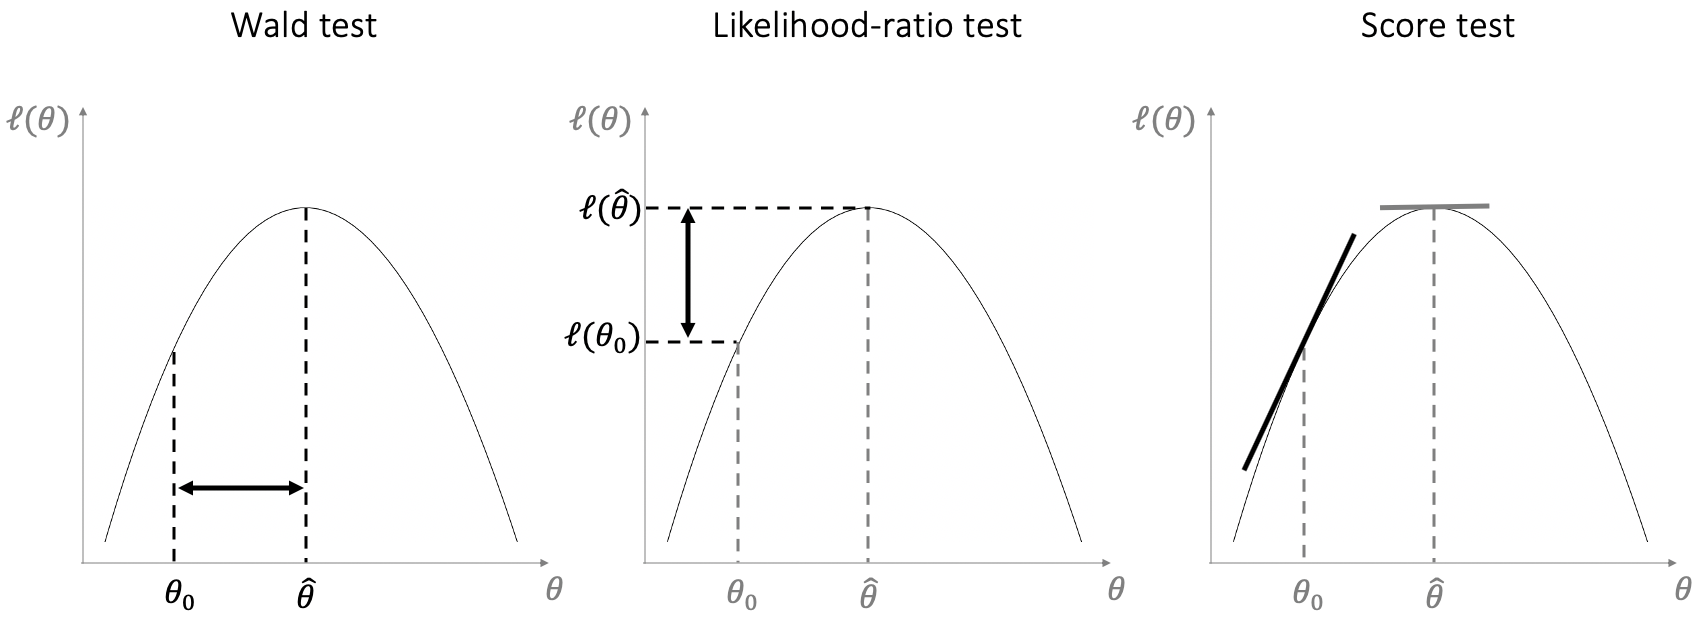
\includegraphics[width=15cm]{Chapter2/Fig/wald_lrt_score_tests.png}
\caption[Wald, LRT and score test]{\textbf{The Wald test, the likelihood-ratio test and the score test}.\\
The three most commonly used statistical testing approaches are illustrated here in the univariate case (single parameter $\theta$). 
On the x axis is the parameter $\theta$, and on the y axis the log likelihood $\ell(\theta)$.
The Wald test essentially evaluates the difference between the \gls{mle} $\hat{\theta}$ and the parameter under $H_0$, $\theta_0$.
The likelihood-ratio test evaluates the difference between the log likelihoods evaluated at those values, i.e. $\ell(\hat{\theta})$ and $\ell(\theta_0)$.
Finally, the score test evaluates the slope of $\ell(\theta)$ at $\theta_0$. Note that the slope at $\hat{\theta}$ is $=0$ by definition, as the MLE maximises $\ell(\theta)$.}
\label{fig:hypothesis_tests}
\end{figure}

\newpage

\subsubsection{Wald test}

First, let us consider the Wald test and the generic null hypothesis $H_0: \boldsymbol{\theta} = \boldsymbol{\theta}_0$ and the alternative $H_1: \boldsymbol{\theta} \neq \boldsymbol{\theta}_0$, where $\boldsymbol{\theta}$ are the parameters in our model and $\boldsymbol{\theta}_0$ are their values under $H_0$.
The Wald test statistic is defined as:

\begin{equation}\label{eq:Wald_test}
W = (\hat{\boldsymbol{\theta}}-\boldsymbol{\theta_0})^T [var(\boldsymbol{\hat{\theta}})]^{-1}(\hat{\boldsymbol{\theta}}-\boldsymbol{\theta_0}), 
\end{equation}

where $\hat{\boldsymbol{\theta}}$ are the MLEs for the $\boldsymbol{\theta}$ parameters (values of $\boldsymbol{\theta}$ that maximise the likelihood).\\

% The XX theorem guarantees that, under some assumptions (ref),
It can be shown that, under some assumptions \cite{wald1943tests}, $W$ follows a chi-squared ($\chi^2$) distribution with number of degrees of freedom (dof) $d$ equal to the number of the parameters tested ($W \sim \chi^2_d $).\\

In the univariate case (d = 1), eq. \eqref{eq:Wald_test} can be expressed as:

\begin{equation}\label{eq:Wald_test_univariate}
    W = \frac{(\hat{\theta}-\theta_0)^2}{var(\hat{\theta})} \sim \chi^2_1.
\end{equation}

Intuitively, our chance of rejecting the null hypothesis increases as the distance between $\hat{\theta}$ and $\theta_0$ increases, and as our confidence in the estimation of the \gls{mle} increases (i.e. $var(\hat{\theta})$ decreases).

\newpage

\subsubsection{Likelihood ratio test}

Second, let us consider the \gls{lrt}.
% It was first introduced by XX. 
Here, the test statistic is the (log) likelihood ratio ($\mathrm{LLR}$):

\begin{equation}\label{eq:log_likelihood_ratio}
\mathrm{LLR} = \log \frac{\mathcal{L}(H_1)}{\mathcal{L}(H_0)} = \ell(H_1) - \ell(H_0), 
\end{equation}

where we compare the value of the log-likelihood of the model under the null and alternative hypotheses, by evaluating eq. \eqref{eq:Linear_regression_log_likelihood} (or eq. \eqref{eq:Linear_regression_log_restricted_likelihood}) using MLE parameters estimated under $H_0$ ($\mathbf{0}$, $\sigma_0^2$) or $H_1$ ($\hat{\boldsymbol{\beta}}$, $\hat{\sigma_1^2}$).  \\

The Wilks theorem \cite{wilks1938large}, under some assumptions, guarantees that $2\mathrm{LLR}$, too, follows a $\chi^2$ distribution with $d$ dof ($2\mathrm{LLR} \sim \chi^2_d$).
The p value can then be calculated as:

\begin{equation}\label{eq:lrt_p_value}
    P(\mathrm{LLR}) = 1-F_{\chi^2}(2\mathrm{LLR}; d).
\end{equation}

\subsubsection{Score test}

Finally the score test, also known as Lagrange multiplier test, is the last hypothesis test we consider. 
It was first developed by Rao in 1948 \cite{rao1948large}.
First, we define the score vector of Fisher as the gradient of the likelihood with respect to its parameters:

\begin{equation}\label{eq:score_vector}
    \mathbf{S} = \frac{\partial \mathcal{L}}{\partial \boldsymbol{\theta}}.
\end{equation}

The score test statistic is the Lagrange Multiplier (LM) and is defined as follows:

\begin{equation}\label{eq:lagrange_multiplier}
    \mathrm{LM} = \mathbf{S}(\boldsymbol{\theta_0})^T [var(\boldsymbol{\theta_0})]^{-1}\mathbf{S}(\boldsymbol{\theta_0}). 
\end{equation}

It can be shown that the $\mathrm{LM}$, too, follows a $\chi^2$ distribution with $d$ dof ($\mathrm{LM} \sim \chi^2_d$).

To understand the intuition behind this test let us consider again the univariate case (d = 1):

\begin{equation}\label{eq:lagrange_multiplier_univariate}
    \mathrm{LM} = \frac{S(\theta_0)^2}{var(\theta_0)} \sim \chi^2_1.
\end{equation}

At the \gls{mle} $\hat{\theta}$, the log likelihood is maximised and therefore its gradient $S(\hat{\theta})$ is equal to $0$.
On the contrary, in principle, $ S(\theta_0) \neq 0 $ (\textbf{Fig. \ref{fig:hypothesis_tests}}). 
Intuitively, the further $ S(\theta_0) $ is away from 0, the more likely we are to reject the null hypothesis.

\newpage

% \subsubsection{Intuition on differences between LRT and score test}
\subsubsection{Intuition on differences between the three tests}

In this thesis, 
% we apply both the \gls{lrt} and the score test, for different applications.
I only apply the \gls{lrt}.
However, for different applications one might want to use alternative approaches.
I use this paragraph to highlight the key differences between the three tests and provide an intuition as to when we should use one or the other.
First of all, it can be shown that \cite{engle1984wald}:

\begin{equation}\label{eq:W_LLR_LM}
    W \geq \mathrm{LLR} \geq \mathrm{LM},
\end{equation}

% Let us exclude the Wald test for this purpose, eq. \eqref{eq:W_LLR_LM} 
which guarantees that the Wald tests statistic is always equal to or greater than the log-likelihood ratio, which in turn is always equal to or greater than the Lagrange multiplier.
The Neyman-Pearson lemma \cite{neyman1933ix} proves that, as a consequence, the power  of the Wald test, defined as the probability of rejecting the null hypothesis when it is false: $P = P($reject $H_0 | H_1)$ (\textbf{Box \ref{box:confusion_mat}}) is the same or higher than the power of the \gls{lrt}, which is the same or higher than the power of the score test:

\begin{equation}\label{eq:power_tests}
    P_W \geq P_{\mathrm{LLR}} \geq P_{\mathrm{LM}}.
\end{equation}

On the other hand, the false positive rate (FPR, \textbf{Box \ref{box:confusion_mat}}) of the \gls{lrt}, defined as the probability of rejecting the null hypothesis when it is true: FPR $= P($reject $H_0 | H_0)$ is also the same or higher than the FPR of the score test (but the same or lower than the Wald test).
The \gls{lrt} can be therefore considered as a good compromise between statistical power and accuracy.
% The score test is therefore the most accurate, making a smaller (or equal) number of Type I errors. \\
Moreover, one advantage of the \gls{lrt} is that it is robust to re-parametrisation of the parameters, whereas the score and Wald tests are not. 
On the other hand, one main 
% One
advantage of the score test is that it does not require the evaluation of the \gls{mle} of the parameters under the alternative hypothesis, but only under the null hypothesis.
\textcolor{blue}{Additionally, while eq. \eqref{eq:power_tests} is generally true, close to the null the score test is considered “locally most powerful”.}
% (ref).
Finally, the $\mathrm{LLR}$ follows a $\chi^2$ distribution (asymptotically) only under the assumptions of the Wilks' theorem, which can be violated in certain applications.
Namely, the value of parameters tested should be far away from the boundaries of the possible values the parameter can assume.
For example, $-\infty < \beta < \infty$, so testing $H_1: \beta \neq 0$ satisfies the assumption.
On the other hand, $0 < \sigma^2 < \infty$ so testing $H_1: \sigma^2 \neq 0$ violates the assumption, because the value $0$ is at the boundary.
Similarly, the score test statistic does not follow a $\chi^2_1$ distribution in the presence of variance parameters, however an alternative test statistic can be defined which follows a linear combination of $\chi^2_1$ distributions, and efficient methods to evaluate its significance have been proposed by Davies \cite{davies1980algorithm}, Kuonen \cite{kuonen1999miscellanea} and Liu \cite{liu2009new, lee2012optimal}. \\

In the analyses in the following chapters (\textbf{Chapters \ref{chapter3}-\ref{chapter5}}), I will use use tests that only evaluate the value of $\beta$, thus the \gls{lrt} is well suited for these applications.
% in the analyses in \textbf{Chapters 
% 3
% \ref{chapter3}-
% % 5
% \ref{chapter5}}, 
% where the tests evaluate $\beta$.
% I use Rao's score test in Chapter 6, where I will be evaluating the variance parameter $\sigma^2$.


\subsection{Correcting the multiple testing burden}
\label{sec:multiple_testing}

In a typical \gls{gwas} one might test hundreds of thousands or millions of genetic variants. 
In e\gls{qtl} mapping, tens of thousands of genes are tested, each essentially equivalent to a \gls{gwas} trait. 
Even when we only test for local e\gls{qtl} (in \textit{cis}, only SNPs within a window around the gene position, see \textbf{section \ref{sec:eqtl}}), we will still test hundreds of variants per gene, taking the average number of tests performed well into the millions.
When performing so many tests, considering single test p values results in a high number of false positives (for example, for p value < 0.05 and 10$^6$ tests we expect 50,000 false positives under the null hypothesis). 
This is known as the `multiple hypothesis testing problem'. 
I use the next section to provide a brief overview of commonly used approaches to correct for multiple hypothesis testing in the context of genetic analysis, with a focus on methods used in e\gls{qtl} mapping.

\subsubsection{Family-wise error rate correction} 

One strategy to perform multiple testing correction is to control the probability of having at least one false positive for a trait, which corresponds to a trait-wise p value known as the family-wise error rate (FWER, \textbf{Box \ref{box:confusion_mat}}).
The widely-used Bonferroni method follows this strategy assuming independence between tests \cite{laird2010fundamentals}. 
Given a desired family-wise significance level $\alpha$, the method consists of calculating `adjusted p values' for each of the un-corrected p values ($P$) as $P_{adj} = P*n $, where n is the number of tests carried out.
Next, setting $P_{adj} < \alpha$ ensures FWER < $\alpha$. 
The Bonferroni correction strategy is conservative, because of the assumption of independence between tests, which ignores correlations between genotypes due to \gls{ld} (\textbf{page \pageref{sec:ld}}).\\

An alternative strategy, which accounts for the dependency of the statistical tests, is to use a permutation-based approach. 
% this below does sound pretty vague
The idea here is to build a background model by drawing from the empirical distribution maintaining the dependency structure of the underlying data but permuting the genotype data across individuals.
This way, we disrupt a possible association between phenotype and genotype whilst maintaining the overall data dependencies. 
% \\
% One first approach is to use permute each SNP M times, and per
For each association test (resulting in an observed p value $p_i$), we can perform the same test M times, each time considering a different permutation of the genotype data across individuals. 
The resulting p values $q_i,m$ represent the null distribution, i.e. the p values we might expect in the absence of any associations.
% \\
One first approach is to use the
% The 
p values from these M additional experiments
% are then used 
to calculate a per-SNP adjusted p value, as the fraction of the M permutation-p values that are lower than the observed p value. 
% \\
For test i, the experimental adjusted p value after M permutations is calculated as:

\begin{equation}\label{eq:permutation_adjusted_pvalue}
    P_{adj,i}^{perm} = \frac{1+\sum_{m=1}^{M} q_{i,m} \geq p_i}{1+M},
\end{equation}

where $q_{i,m}$ is the p value obtained at the m$^{th}$ permutation run equivalent to test i, and ones are added to avoid zero divisions.  
This strategy accounts for local \gls{ld}, thereby increasing the statistical power, and has been widely used in $cis$ molecular \gls{qtl} mapping to estimate gene-level p values \cite{gtex2015genotype, sudmant2015integrated}. 
% \\
% rephrase this
% Second, significant p values are truncated to a limited level of significance determined by the number of permutations. For example, 10,000 permutations restrict the p values to a lower bound of $10^{-4}$. Typically, one will obtain a list of genes that have the same lower-bound p values, such as $10^{-4}$. However, it is desirable to know the exact significance of each eGene p value for better interpretation and prioritisation of genes.
However, as evident from eq. \eqref{eq:permutation_adjusted_pvalue}, the lower bound of $P_{adj,i}^{perm}$ depends on the number of selected permutations\footnote{For example, for M=1,000 the smallest adjusted p value we can obtain is only $P_{adj,i}^{perm}$=0.001 (when no permuted p value is smaller than the p value observed).} for which the test statistic is calculated, and thus a higher number of permutations may be required to estimate a p value with high enough accuracy \cite{sul2015accurate}.
This can be improved by increasing the number of permutations, e.g. using M as large as 100,000, but that entails a great computational burden and can become unpractical in molecular analyses of large cohorts.
\\

A second approach is to adjust for multiple testing when considering a more complex hypothesis, for example by pooling across variants, thus requiring fewer permutations.
% I am wondering are you creating a new test which is to identify the minimal p-value for the region and want to correct this using permutations? 
As an example, in the method described in \cite{ongen2016fast}, the minimal p values for each permutation across all SNPs are selected, and used to build a beta distribution of background p values, against which to compare the real p values.
% Recently, one method has been developed that uses permutation results for as little as (M=) 50-100 permutations to estimate a full distribution of background permuted p values, 
This method has been shown to robustly work for as little as (M=) 50-100 permutations, making use of the benefits of the assumption-free permutation approach without too much of the computational burden \cite{ongen2016fast}. 
This is the method I will use in the following chapters (\textbf{Chapters \ref{chapter3}}, \textbf{\ref{chapter4}} and \textbf{\ref{chapter5}}) of this thesis to control for FWER at gene level when performing large scale \gls{eqtl} mapping.

\subsubsection{False discovery rate correction}

An alternative solution for multiple testing correction is to control the \gls{fdr}, i.e. the expected percentage of false discoveries (\textbf{Box \ref{box:confusion_mat}}).
The most widely used FDR-based correction method is the Benjamini-Hochberg (BH) procedure \cite{benjamini1995controlling}, which again assumes independence between tests\footnote{\textcolor{blue}{Although, more recently, the BH procedure has actually been shown to hold under positive dependency \cite{benjamini2001control}.}}. 
Let us consider T tests with p values $p_1, p_2, ..., p_T$ and let $r_1, r_2, ..., r_T$ be their ranks (the smallest p value has rank 1, the largest has rank T), defining adjusted p values as $P_{adj,i} = \frac{T*p_i}{r_i} $ and setting $P_{adj,i} <\alpha$ ensures FDR < $\alpha$ \cite{yekutieli1999resampling}.
Alternatively, the Storey procedure (proposed in 2002 \cite{storey2002direct, storey2003statistical}) optimises the BH procedure by taking into account the distribution of the p values in the experiment.
% \\
FDR-corrected p values 
% using the Storey procedure 
are sometimes called `q values'.
% \\
% add intuition behind FWER/FDR?
For \gls{eqtl} mapping, the assumption of independent tests holds when we consider a single \gls{snp} per gene.
In this case, the number of tests T coincides with the numbers of genes tested.
In practice, in most applications one is interested in the lead \gls{snp} for each gene, i.e. the \gls{snp} corresponding to the minimum p value.
Conditional analyses (where we include the top \gls{snp} as a covariate in the model) can be used subsequently to detect secondary and tertiary effects for a gene.

\subsubsection{Multiple testing correction for \textit{cis} e\gls{qtl} mapping}

A typical strategy to correct for multiple hypothesis testing in \textit{cis}-e\gls{qtl} mapping is to use a two-step procedure \cite{gtex2015genotype}. 
First, for each gene an experiment-wise p value is obtained by correcting for multiple testing across variants using a FWER-based method. 
These gene-level p values are probability values for the hypothesis of a gene having at least one e\gls{qtl} in the analysed region (i.e. of being an eGene). 
Second, the gene-level p values are corrected to control the FDR, for example using the Benjamini-Hochberg procedure.\\

In the analyses in \textbf{Chapters 3-5} of this thesis, I adopt this two-step approach.
I use M=1,000 permutations and the method described in \cite{ongen2016fast} to correct p values at the gene level (I will call the p values obtained this way `empirical feature p values').
Then, I select the top \gls{snp} per gene and correct the corresponding empirical feature p values a second time, using the Storey procedure \cite{storey2002direct}.
I will call the resulting p values: `globally corrected p values'.

\subsection{Calibration studies and distributions of p values}

Under the assumption of no association between genetic variants and the analysed trait, an association model is expected to produce p values that approximately follow a uniform distribution.
If that is the case, the model is said to be `calibrated'.
To verify that a model is calibrated we can disrupt the association between genotypes and phenotypes, by randomly permuting the genotypes. 
A representation that is often used to compare the observed (permuted) and the expected distributions of p values is the \gls{qq} plot. 
In a \gls{qq} plot the observed negative $\log_{10}$(p value) is plotted against the expected negative $\log_{10}$(p value), where the expected value is obtained by drawing from a uniform distribution. 
I define as `confounding', variables that are correlated with the genotype $\mathbf{g}$ (and sometimes also the phenotype $\mathbf{y}$) and thus may create spurious associations when left unaccounted for (see also \textbf{section \ref{sec:linear_mixed_models}}).
Inflated \gls{qq} plots are typically associated with the presence of such confounding factors, and can be used as a diagnostic tool (\textbf{Fig. \ref{fig:qqplots}}). 

% \vspace{2mm}

\begin{figure}[h]
\centering
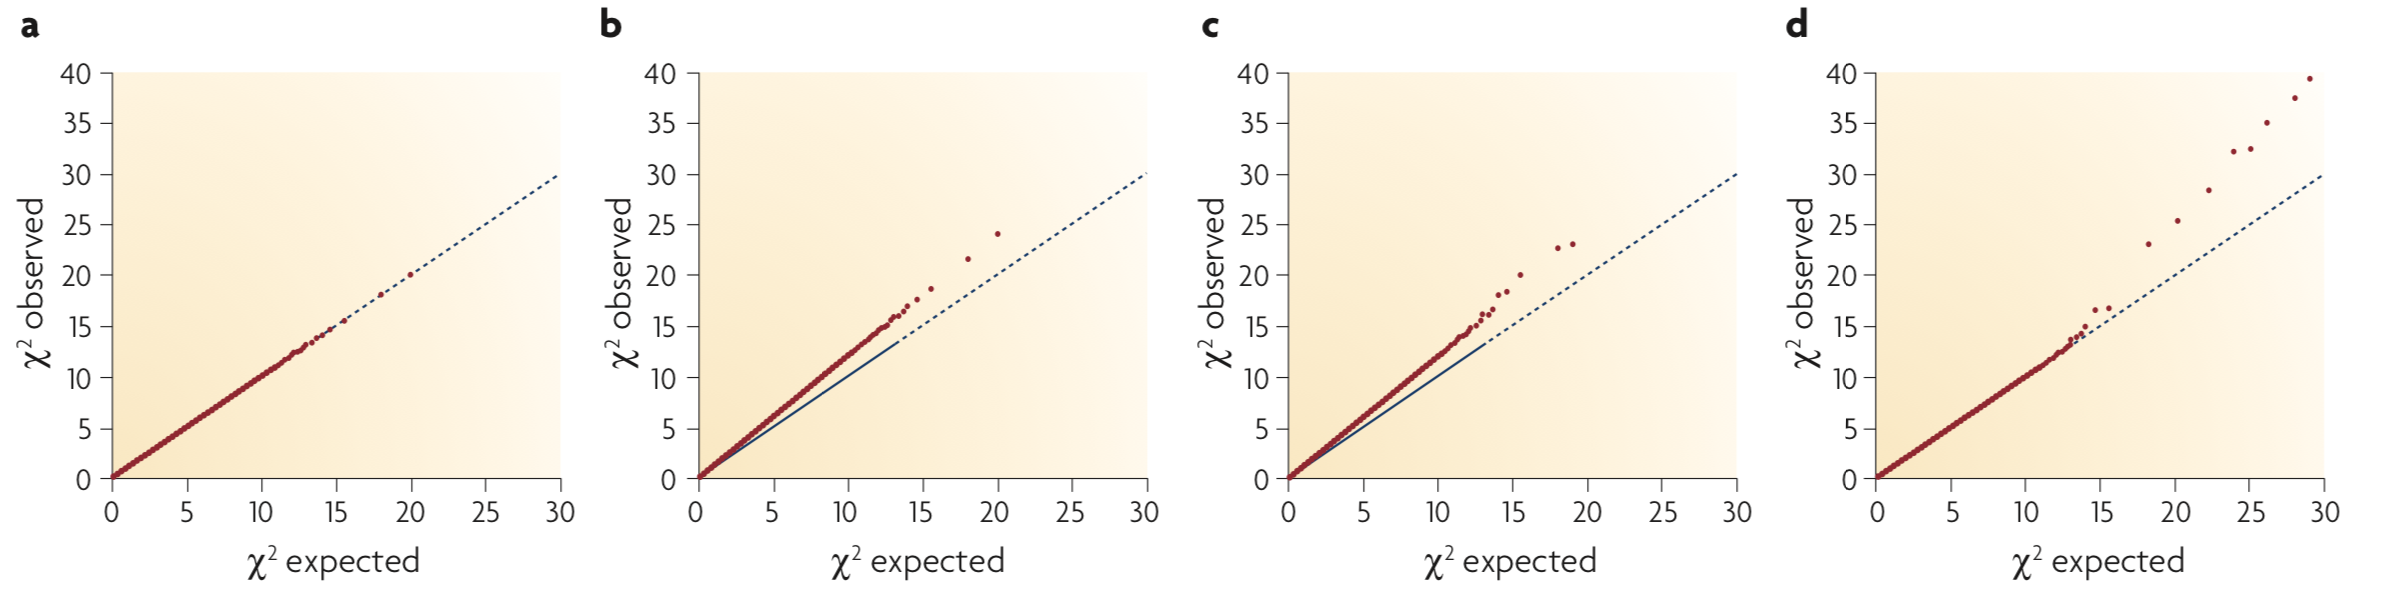
\includegraphics[width=15cm]{Chapter2/Fig/qqplots.png}
\caption[QQ plots]{\textbf{Example QQ plots}.\\
Examples of quantile-quantile (QQ) plots, displaying the expected negative log p values (x axis) versus the observed negative log p values (y axis) under the null hypothesis (diagonal blue line) and observed (red circles) in (a) when no associations are present, such that there is no departure from the null distribution,  (b) in the presence of confounding factors, such that there is constant departure from the null distribution and (c) in the presence of a genuine genetic association, such that there is departure from the null in the tail of the distribution.
Adapted from 
% McCarthy et al.
% Placeholder adapted from
\cite{mccarthy2008genome}.
% (a) no association (b) cryptic relatedness (c) population stratification (d) genuine association - 
% Change this to real data and -$\log_{10}$(p value) rather than $\chi^2$ (possibly remove one between b and c)
}
\label{fig:qqplots}
\end{figure}

% \clearpage

% discuss two types of confounders

% \subsection{Confounding effects in linear model}
\subsection{Including covariates in a linear model}
\label{sec:confounders}

The model in eq. \eqref{eq:Linear_regression_genetics} models the \gls{snp} tested as the only factor affecting the measured phenotype.
However, if available, additional relevant information for the samples tested (such as the sex or the age of the individuals) can be added to the model as covariates ($\mathbf{W}$), and often improve discovery power by controlling for additional phenotypic variation. 
The model becomes:

\begin{equation}\label{eq:Linear_regression_genetics_covariates}
 \mathbf{y} =  \mathbf{W}\boldsymbol{\alpha} + \mathbf{g}\beta + \boldsymbol{\psi}, 
\end{equation}

where $\mathbf{W}$ is an $N \times P$ matrix whose columns are known covariates, and $\boldsymbol{\alpha}$ is a $P \times 1$ vector of the corresponding weights.
Here, covariates are implemented as fixed effects (FEs), and they only contribute to the mean value of $\mathbf{y}$, such that $E[\mathbf{y}] = \mathbf{W}\boldsymbol{\alpha} + \mathbf{g}\beta$, while $Var(\mathbf{y}) = Var(\boldsymbol{\psi}) = \sigma_n^2 \mathbf{I_N} $, as before.
In some cases, we can add FE covariates to adjust for
% other confounding, such as 
technical batches
% and other experimental conditions 
or other factors that might 
affect $\mathbf{y}$, 
increasing the accuracy of our model.
% and thus skew the results. 
% \\
In \gls{eqtl} mapping, we can often take advantage of the 
full transcriptome
% expression profiles across all genes 
to identify 
% global
% confounding 
factors
affecting
gene expression in a global manner, 
thus efficiently capturing known and potentially hidden covariates affecting expression across all genes.
% even when we do not necessarily know the origin of the confounding.
For example, we can perform principal component analysis (PCA) on the full expression matrix (genes x samples) and include such expression PCs as covariates in the model.
Alternative more sophisticated methods to compute factors capturing global trends include, among others,
% surrogate variable analysis (
SVA \cite{leek2007capturing}, 
% probabilistic estimation of expression residuals (
PEER \cite{stegle2010bayesian, stegle2012using},
% factorial single cell latent variable model (
f-scLVM \cite{buettner2017f},
% probabilistic Count Matrix Factorization (
pCMF \cite{durif2019probabilistic},
% single cell variational inference (
scVI \cite{lopez2018deep, svensson2020interpretable}
% , both in its standard \cite{lopez2018deep} and linear \cite{svensson2020interpretable} version,  
% probabilistic analysis of genomic data (PANAMA) \cite{fusi2012joint} 
and 
% multi-omics factor analysis (
MOFA \cite{argelaguet2018multi}. 
% \\

\textcolor{blue}{Different approaches can be used to determine the optimal number of PCs (or other factors) to include in the model.
A popular approach is to choose the number of factors that maximises the number of eQTL discoveries \cite{westra2014genome, gtex2017genetic, aguet2019gtex}.
The assumption is that global effects captured by PCs are orthogonal to the effects of a single variant on the expression of one gene, and thus there is no risk of generating false positives. 
There remains however a risk of over-correction, which can introduce synthetic associations as a result of collider bias \cite{aschard2017covariate}.
% This is the approach used in this thesis.
Alternatively, 
% one could determine the number of optimal PCs to include based on the cumulative variance explained (e.g. at least 50\%), while not exceeding XX (sample size available) to retain sufficient degrees of freedom. 
% Finally, 
to verify that specific covariates of interest (not modelled explicitly) are accounted for in the PCs, one may verify that PCs explain enough variance for those covariates (see for example the analysis I describe in \textbf{Chapter \ref{chapter5}, section \ref{sec:neuroseq_eqtl_methods}}).}


\begin{figure}[htbp]
\centering
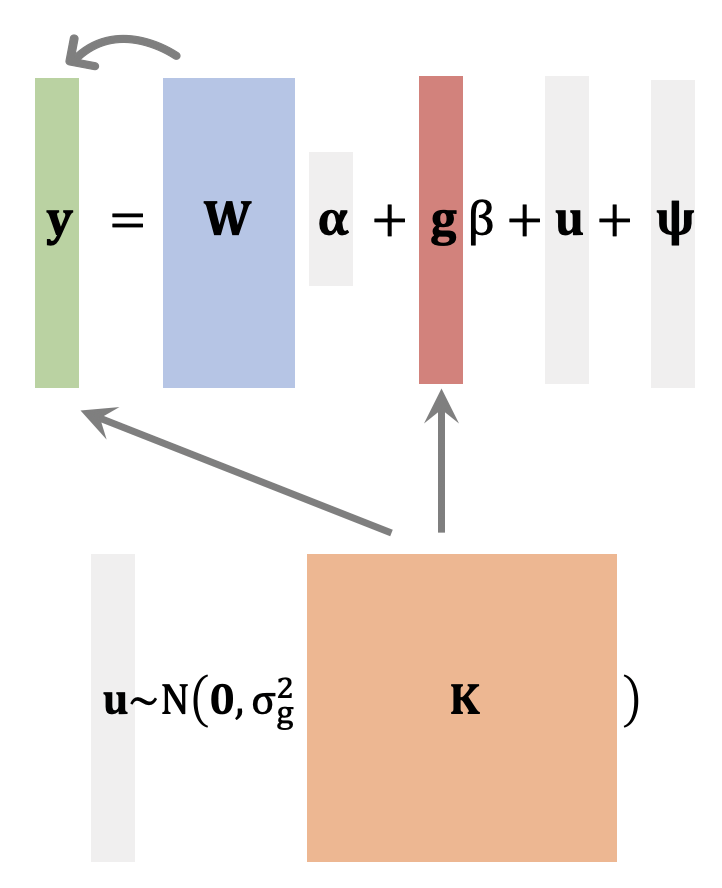
\includegraphics[width=10cm]{Chapter2/Fig/confounders_covariates.png}
\caption[Confounders and covariates]{\textbf{Confounders and covariates}.\\
Traditionally `confounders' are variables that are correlated with both the genotype vector and the phenotype, i.e. hidden common causes of both $\mathbf{g}$ and  $\mathbf{y}$. 
For example, population structure ($\mathbf{K}$) is a confounder in population genetics studies. 
On the other hand, other covariates such as sex (unless we are testing genes on the X or Y chromosomes) and batch ($\mathbf{W}$), only have an effect on $\mathbf{y}$.
By including them as covariates in the model, we control for additional phenotypic variation and thereby increase association power. 
We note that in the illustration, a linear mixed model is used to illustrate how to account for both effects, with a random effect term used to correct for population structure, and covariates included as fixed effects. 
However, mathematically, both can be treated in the same way (i.e. they both can be included as fixed or random effects). 
In contrast the motivation for including them, and the effect their inclusion has, are different.}
\label{fig:conf_cov}
\end{figure}
% \newpage

%********************************** %Third Section  **************************************

\section{Population structure and linear mixed models}
\label{sec:linear_mixed_models}

One major source of confounding effects in genetic analysis - that I have purposefully not discussed thus far -  is latent population substructure, which includes population stratification (i.e. the presence in the study sample of individuals with different ancestral and demographic histories) and relatedness between individuals, both known relatedness (e.g. known familial relations within a sample) and \textcolor{blue}{cryptic relatedness (i.e. evidence that individuals in the study sample have residual, non-trivial degrees of relatedness) \cite{mccarthy2008genome}.}
It was acknowledged, even before the first \gls{gwas} was conducted, that there was a possibility of identifying false positives (or that true positives may be masked) when using population based association studies (instead of family based linkage studies), due to those confounding effects \cite{burton2005key}. 
This is because both phenotypic prevalence (proportion of individuals exhibiting the phenotype) and allele frequencies (frequencies of a specific allele within a population) vary across different populations, which may result in the identification of spurious association between variants and the phenotype of interest due to ethnicity or population sub-structure (including relatedness) \cite{burton2005key} (\textbf{Fig. \ref{fig:conf_cov}}).

% name examples
% and mention differences as compared to covariates: pop struct affects both y and g

\subsection{Early approaches to account for population structure}
\label{sec:pop_struct_noLMM}

Various approaches have been proposed to account for population structure.
An early solution was genomic control \cite{devlin1999genomic}.
Genomic control correction adjusts for inflation due to confounding effects by dividing the test statistic of each marker by the genomic control parameter ($\lambda_{GC}$\footnote{$\lambda_{GC}$ compares the test-statistic value with the median value, such that $\lambda_{GC} \approx 1$ means there is no evidence for confounding, $\lambda_{GC} \gg 1$ indicates that the presence of confounding is likely.}). \\

\newpage

However, as different markers have different abilities to distinguish between populations, this uniform adjustment is far from optimal. 
Indeed, as a result, markers that strongly segregate across different population groups are only partially corrected, whereas markers that do not segregate tend to be over-corrected \cite{marchini2004effects, price2006principal}.
Alternatively, a method that attempts to correct the underlying problem is STRUCTURE, which assigns individuals to discrete population subgroups and then combines the evidence for association across the different subgroups \cite{pritchard2000inference}. 
A limitation of this method is that only discrete subgroups can be considered. 
Additionally, it does not scale with sample size and is also highly sensitive to the number of defined population clusters \cite{price2006principal}.\\

The analysis of genotype data from large population studies, showed that genome-wide genetic variation could be used to
accurately infer population structure 
% Bauchet 2007, Jakobsson 2008, 
\cite{li2008worldwide, tian2008analysis, price2008discerning}.
In particular, it could be shown that the first principal components (PCs) calculated from the genotypic data were correlated with geographic axes \cite{novembre2008interpreting}.
As a result, one approach to account for population structure is to add the first genotypic PCs as covariates in the model (or to regress them out \cite{price2006principal}): 

\begin{equation}\label{eq:LM_PC_confounding}
    \mathbf{y} =  \mathbf{W}\boldsymbol{\alpha} + \sum_{i=1}^{p} PC_i b_i + \mathbf{g}\beta + \boldsymbol{\psi}. 
\end{equation}

The number of leading PCs p can be determined as the number of \gls{pc}s that cumulatively describe a certain proportion of the total genotypic variance.
% , or ..
This approach (eq. \eqref{eq:LM_PC_confounding}) was shown to perform relatively well in removing global population structure, but often failed to detect the more subtle relatedness effects.
Therefore, when PCs are used to correct for population structure, closely related individuals have to be removed from the association analyses, prior to PCA calculations.
Even then, cryptic relatedness might still be present and would not be properly accounted for by this method. 

% \newpage

\subsection{Linear mixed models for genetic analyses}
\label{sec:LMM}

\textcolor{blue}{Alternatively, linear mixed models (LMMs) can be used to successfully account for confounding effects linked to both population stratification and cryptic relatedness 
\cite{yu2006unified, kang2008efficient,kang2010variance, price2010new, zhou2012genome, lee2018genome}.}
In an LMM, istead of being used to calculate principal components, the genotype data is used directly to estimate an $N \times N$ kinship matrix, $\mathbf{K}$, that describes the genetic similarity between pairs of individuals (see section below for a description of commonly used approaches to generate $\mathbf{K}$). \\

This genetic similarity is modelled through the use of an additional random effect term in the linear model described by eq. \eqref{eq:Linear_regression_genetics_covariates}, as follows:

\begin{equation}\label{eq:Linear_mixed_model}
 \mathbf{y} =  \mathbf{W}\boldsymbol{\alpha} + \mathbf{g}\beta + \mathbf{u} + \boldsymbol{\psi}, 
\end{equation}

where $\mathbf{u} \sim \mathcal{N}(\mathbf{0}, \sigma_g^2\mathbf{K})$.
The use of the notation $\mathbf{K}$ signifies the fact that this matrix reflects a degree of `kinship' between individuals. 
It can be shown that the LMM approach is theoretically equivalent to the PC
approach when all PCs are regressed or included as covariates (see Hoffman \textit{et al.} \cite{hoffman2013correcting} for details), explaining why LMMs are able to account for more subtle population structure than the PC approach. 
However, regressing all PCs or including all PCs as covariates is not feasible in practice (as the number of variables would exceed that of observations). 
% \\

% The model in eq. \eqref{eq:Linear_mixed_model} can be alternatively expressed as:

% \begin{equation}\label{eq:LMM_MVN}
%  \mathbf{y} \sim  \mathcal{N}(\mathbf{W}\boldsymbol{\alpha} + \mathbf{g}\beta, \sigma_g^2\mathbf{K} + \sigma_n^2\mathbf{I}).
% \end{equation}

% Note that for ease of notation in the following equations I have dropped the subscript $N$ from the identity matrix (i.e. $\mathbf{I} = \mathbf{I}_N$).

% Ideally, if we knew the underlying sub-population structure of our samples and could pinpoint which variants showed different allele frequencies within the population of interest, we could simply include such variants as covariates (i.e. similar to $\mathbf{W}$ from eq. \eqref{eq:Linear_regression_genetics_covariates}):

% \begin{equation}\label{eq:LM_G_confounding}
%     \mathbf{y} =  \mathbf{W}\boldsymbol{\alpha} +  \mathbf{G}_{conf}\mathbf{b}_{conf} + \mathbf{g}\beta + \boldsymbol{\psi}, 
% \end{equation}

% where $\mathbf{G}_{conf}$ is a matrix with columns corresponding to the genotypes of the \gls{snp}s whose frequencies vary within a population and thus cause confounding effects, and $\mathbf{b}_{conf}$ are the corresponding weights. 
% However, this is not typically the case.
% In fact, Fisher's work showed that it is the infinitesimal additions of a large number (if not all) of genetic variants that contributes to population structure \cite{fisher1919xv} .

% Alternatively, \gls{lmm}s can be used to successfully account for confounding linked to latent population structure.
% The intuition is to consider eq. \eqref{eq:LM_G_confounding}, but this time considering \gls{snp}s from the whole genome, since we do not know the `confounding variants':

% \begin{equation}\label{eq:polygenic_model}
%     \mathbf{y} =  \mathbf{W}\boldsymbol{\alpha} +  \mathbf{G}\mathbf{b} + \mathbf{g}\beta + \boldsymbol{\psi}.
% \end{equation}

% This is called the `polygenic model' (ref).
% Now, if we assume that the weights $\mathbf{b}$ are drawn from a common normal distribution $\mathbf{b} \sim \mathcal{N}(\mathbf{0},\sigma^2_g\mathbf{I_M})$, where $M$ is the total number of \gls{snp}s, it can be shown that:

% \begin{equation}\label{eq:LMM_u_confounding}
%     \mathbf{u} =  \mathbf{G}\mathbf{b} \sim \mathcal{N}(\mathbf{0},\sigma^2_g, \mathbf{G}\mathbf{G}^T)
% \end{equation}

% where $\mathbf{u}$ is a random variable which captures the effect of latent population structure onto $\mathbf{y}$.
% The model we just described is a \gls{lmm}.\\

% In terms of removing effects of population stratification, \gls{lmm}s have been shown to perform as well as  including all M PCs (or regressing them out, \cite{price2006principal}), which is of course not feasible in practice.
% Additionally, \gls{lmm}s successfully correct for more subtle effects due to cryptic relatedness.
% However, \gls{lmm}s are typically much more computationally demanding.
% The next section describes \gls{lmm}s in general and introduces fast implementation approaches for a specific class of \gls{lmm}s.

% \subsection{Linear mixed models}

% % gwas reference: \cite{bush2012genome}

% In a \gls{lmm} the outcome variable can be described as a sum of deterministic effects (fixed effects, FE) and random effects (RE).
% % A random effect is ..
% A \gls{lmm} can be expressed as:

% \begin{equation}\label{eq:Linear_mixed_model_general}
%  \mathbf{y} =  \mathbf{W}\boldsymbol{\alpha} + \mathbf{Z}\mathbf{b} + \boldsymbol{\psi}, 
% \end{equation}

% where $\mathbf{y}$ is the outcome variable, $\mathbf{W}$ and $\mathbf{Z}$ are the design matrices of fixed and random effects respectively; $\boldsymbol{\alpha}$ are the fixed effects, $\mathbf{b} \sim \mathcal{N}(\mathbf{0},\sigma_b^2\boldsymbol{\Sigma_b})$, $\boldsymbol{\Sigma_b}$ is a known covariance matrix, $\boldsymbol{\psi} \sim \mathcal{N}(\mathbf{0},\sigma_n^2\mathbf{I})$ is the noise vector and $\sigma_b^2$ and $\sigma_n^2$ are the variance parameters of the random effect and the noise, respectively.\\

% In contrast to the case of linear regression discussed in section \ref{sec:linear_regression}, there is no close-form solution for the (restricted) \gls{mle} of the model parameters. \\

% However, for the model in eq. \eqref{eq:LMM_u_confounding} (i.e. when $\boldsymbol{\Sigma_b}$ factors as $\mathbf{G}\mathbf{G}^T$) it is possible to speed up computations, provided that we can perform feature selection on genomic variants and therefore make the genetic relatedness matrix low rank \cite{lippert2014greater}: 




\subsubsection{Kinship matrices}
\label{sec:kinship_matrices}

The covariance matrix $\mathbf{K}$ captures the latent population sub-structure of the samples considered, including population stratification and genetic relatedness.
% \\
Several approaches have been proposed to compute this matrix, which is sometimes called the genetic relatedness matrix (GRM).
% \\
Fisher’s infinitesimal model (see \textbf{section \ref{sec:Fisher}}) \cite{fisher1919xv} demonstrated that under an additive model with an infinite number of infinitesimal genetic effects, the phenotype follows a normal distribution, and the correlation of phenotypes between individuals is proportional to the fraction of genetic material that is `identical-by-descent' (IBD)\footnote{A genetic locus is IBD between two individuals if it has been inherited by a common ancestor.}. 
A consequence of this observation is that we can define the genetic relatedness between two individuals by using the predicted proportion of the genome that is IBD between them. 
Traditionally, an IBD (relatedness) matrix was estimated using known pedigrees (see \textbf{Box \ref{box:genetic_terms}}) \cite{lange1976extensions}. 
% Note that the definition of IBD requires the specification of a base population (i.e. the ancestors, which are assumed to have average relationship equal to zero), which in the case of pedigree designs is the population of the founders \cite{powell2010reconciling}.
\\

An alternative, increasingly popular solution is to estimate the relatedness matrix using genome-wide SNPs. 
The use of SNP-based relatedness matrices improves
% narrow-sense
heritability estimates \cite{visscher2006assumption, visscher2007genome, hayes2009increased} and allows the user to better account for population structure \cite{kang2008efficient, lee2010using} compared to pedigree-based matrices. 
Different ways of estimating relatedness matrices from genotype data have been proposed \cite{oliehoek2006estimating, purcell2007plink, vanraden2008efficient}. 
Finally, a commonly-used approximation of the GRM is the `realised' relatedness matrix ($\mathrm{RRM}$) \cite{hayes2009increased}, which is defined as:

 \begin{equation}
    \mathrm{RRM} = \frac{1}{M}\mathbf{G}\mathbf{G}^T,
\end{equation}

where $\mathbf{G}$ is the $N \times M$ genotype matrix with standardised genotypes across individuals and $M$ denotes the number of genome-wide variants. 
The $\mathrm{RRM}$ can be directly obtained from the polygenic model (where many genetic variants contribute to the trait):

\begin{equation}\label{eq:polygenic_model}
    \mathbf{y} \sim N (\mathbf{W}\boldsymbol{\alpha} +  \mathbf{G}\mathbf{b}, \sigma_e^2\mathbf{I}),
\end{equation}

where $\mathbf{b}$ is an $M \times 1$ vector containing the weights corresponding to $\mathbf{G}$ defined as above (standardised genotype matrix).
If we assume that $\mathbf{b}$ is drawn from a normal distribution such that: $\mathbf{b} \sim \mathcal{N}(\mathbf{0}, \frac{\sigma_g^2}{M} \mathbf{I_M})$\footnote{Note that each genetic marker explains on average variance $\frac{\sigma_g^2}{M}$, so that genome-wide variants jointly explain variance $\sigma_g^2$.}, and marginalising out the random effect we obtain the RRM in one of the terms of the covariance:

\begin{equation}\label{eq:polygenic_model_MVN}
    \mathbf{y} \sim N (\mathbf{W}\boldsymbol{\alpha}, \sigma_g^2\frac{1}{M}\mathbf{G}\mathbf{G}^T + \sigma_e^2\mathbf{I} ),
\end{equation}

The $\mathrm{RRM}$ can also be interpreted as an IBD relatedness matrix where the base population
is the current population \cite{powell2010reconciling}. 
% \\
Throughout this thesis, we use the $\mathrm{RRM}$ described in \cite{yang2011gcta} as implemented in PLINK \cite{purcell2007plink}.


% Hayes et al. 74 
% \subsubsection{Relationship to PCs}

% Principal components of the genotype data G can be calculated as the eigenvectors of the relatedness matrix $\mathbf{K} = \frac{1}{M}\mathbf{G}\mathbf{G}^T$\cite{price2006principal}. 
% Denoting with $\mathbf{Q}\mathbf{S}\mathbf{Q}^T$ the eigenvalue decomposition6 of $\mathbf{K}$, the marginalised model in eq. \eqref{eq:polygenic_model_MVN} can be obtained from the linear mixed model

% \begin{equation}
%     \mathbf{y} \sim N (\mathbf{W}\boldsymbol{\alpha} +  \mathbf{U}\mathbf{b}, \sigma_e^2\mathbf{I}),
% \end{equation}

% with $\mathbf{b} \sim \mathcal{N}(\mathbf{0}, \sigma_g^2\mathbf{S})$
% by integrating out the random effects $\mathbf{b}$. 
% In summary, while a PC-based linear model only accounts for the first principal components of the genotype data using fixed effects, linear mixed models consider all the principal components using random effects. 
% This explains why LMMs can account for more subtle (i.e. high-rank) confounding compared
% to PC-based linear models. For further details on the relationship between PC-based
% models and random effect models I refer to Hoffman \cite{hoffman2013correcting}.

% \newpage

\subsection{Fast implementation of LMMs}
\label{sec:fast_lmm}

The biggest limitation of the use of LMMs for association studies is that they are in general very computationally intensive.
Computations associated with the parameter inference in LMMs scale cubically with
the number of individuals in the dataset. 
Indeed, for the generic LMM
the evaluation of the (restricted) marginal likelihood entails the computation of operations with $\mathcal{O}(N^3)$ complexity, specifically the inversion and the determinant of the total covariance. % remove if add the following
% :
% \begin{equation}
%     \mathbf{y} \sim \mathcal{N}(\mathbf{X}\boldsymbol{\beta}, \mathbf{K_{\theta}})
% \end{equation}
% (where $\mathbf{K_{\theta}}$ etc), 
% the evaluation of the restricted marginal likelihood:
% \begin{equation}
%     L = - \frac{N-F}{2} \log (2\pi) - \frac{1}{2} \log \det \mathbf{K_{\theta}} - \log \det \mathbf{X}^T\mathbf{K_{\theta}}^{-1}\mathbf{X}
% \end{equation}
% where $\boldsymbol{\beta}_{\theta} = (\mathbf{X}^T\mathbf{K_{\theta}}^{-1}\mathbf{X})^{-1}\mathbf{X}^T\mathbf{K_{\theta}}^{-1}\mathbf{y}$\\
% entails the computation of operations with $\mathcal{O}(N^3)$ complexity, specifically the inversion and the log determinant of the total covariance.
However, for the model in eq. \eqref{eq:Linear_mixed_model}, i.e. when the covariance matrix is known (does not depend on any parameters), and which can be alternatively expressed as:

\begin{equation}\label{eq:LMM_MVN}
 \mathbf{y} \sim  \mathcal{N}(\mathbf{W}\boldsymbol{\alpha} + \mathbf{g}\beta, \sigma_g^2\mathbf{K} + \sigma_n^2\mathbf{I}),
\end{equation}

it is possible to speed up computations \cite{kang2008efficient, kang2010variance, lippert2011fast, zhou2012genome} ,thus enabling application to large population studies. 
These stratagems reduce the computational complexity from $\mathcal{O}(N^3)$
per-SNP to a single  $\mathcal{O}(N^3)$ cost upfront, and a per-SNP complexity of  $\mathcal{O}(N^2)$.
The complexity can be further reduced to $\mathcal{O}(N^2)$ for the upfront computation and a per-test complexity of  $\mathcal{O}(N)$, provided the genetic relatedness matrix is low-rank. 
% \\
% In practice, this can be achieved through a feature selection approach, selecting a small proportion of all genome-wide variants to estimate $\mathbf{K}$ \cite{listgarten2012improved} or by randomly selecting a subset of the genome-wide variants. 
% As I will show in Section 2.3.3, an efficient derivative-free inference scheme can be used for association testing in univariate models 
% % \cite{}. 
% However, the number of variance parameters in variance component analyses and multi-trait models is typically too large for the efficient use of derivative-fee methods. 
% Multiple optimisation schemes have been proposed to optimise the restricted marginal likelihood in these cases
% However, in recent years, a lot of research has focused on methods to improving the efficiency of these methods.
% Whilst naively the LMM scales cubically with the number of samples, there are now methods available that scale linearly with the number of samples, once some up front computations that scale quadratically with the number of samples have been performed.
% These include FaST-LMM \cite{lippert2011fast}, BOLT-LMM \cite{loh2015efficient} and LIMIX \cite{lippert2014limix}, the latter built using a flexible framework such that different types of testing procedure can be easily and efficiently implemented, including interaction tests (see section \ref{sec:lmm_gxe}).\\
% FaST-LMM, BOLT-LMM, LIMIX.
% , including first-derivative methods, such as expectation maximisation (EM, Dempster et al., 1977) and its improved version PX-EM (Liu et al., 1998; Foulley and Van Dyk, 2000), and second-derivative methods, such as the Newton-Ralphson algorithm (Zhou and Stephens, 2014), the average information REML algorithm (Gilmour et al., 1995) and the Broyden’s method (Groeneveld, 1994). In this thesis, we follow (Groeneveld, 1994) and consider the Broyden’s method for parameters inference. 
% For a discussion on the different optimisation algorithms for inference in \gls{lmm}s, I refer to the supplementary information of Loh et al. (2015a).

\newpage

I use this section to  briefly describe the efficient FaST-LMM algorithm proposed by Lippert \textit{et al} \cite{lippert2011fast}.
This is the algorithm implemented within the LIMIX toolset \cite{lippert2014limix,casale2015efficient} which I use throughout this thesis.
\\

The intuition is to project all data into a space where phenotypic variables ($\mathbf{y}$) and covariates ($\mathbf{W}, \mathbf{g}$) are uncorrelated so that 
% the parameters 
in the rotated 
space the joint system to estimate the optimal model parameters 
% data 
can be solved in closed-form.
% , i.e. with a diagonal covariance matrix. 
To do so, we perform eigen decomposition of $\mathbf{K}$ from eq. \eqref{eq:LMM_MVN}, such that: $\mathbf{K} = \mathbf{Q}\mathbf{S}\mathbf{Q}^T$, where $\mathbf{S}$ is a diagonal matrix containing the eigenvalues of $\mathbf{K}$ on the diagonal and zeroes elsewhere, and $\mathbf{Q}$ is orthonormal ($\mathbf{Q}\mathbf{Q}^T = \mathbf{I}$), with columns corresponding to the eigenvectors of $\mathbf{K}$. 
% \\
Then, if we define $\delta = \sigma_n^2/\sigma_g^2$ and consider it fixed, the full covariance matrix can be expressed as:

\begin{equation}\label{eq:fast_lmm_full_covariance}
 Var(\mathbf{y}) = \sigma_g^2\mathbf{K} + \sigma_n^2\mathbf{I} = \sigma_g^2(\mathbf{Q}\mathbf{S}\mathbf{Q}^T + \delta\mathbf{I})= \sigma_g^2\mathbf{Q} (\mathbf{S} + \delta\mathbf{I})\mathbf{Q}^T.
\end{equation}

\vspace{4mm}

To simplify notation, we use $\boldsymbol{\Sigma} = \mathbf{K} + \delta\mathbf{I}$; $\mathbf{X} = [\mathbf{W}, \mathbf{g}$] and $\boldsymbol{\beta} = [\boldsymbol{\alpha}, \beta]$, such that we can express the full log-likelihood as:

\begin{equation} \label{eq:fast_lmm_log_likelihood}
 \ell(\boldsymbol{\beta}, \sigma_g^2, \delta) = -\frac{1}{2} \bigg\{N\log(2\pi\sigma_g^2) + \log{|\boldsymbol{\Sigma}|}+ \frac{1}{\sigma_g^2}(\mathbf{y}-\mathbf{X}\boldsymbol{\beta})^T\boldsymbol{\Sigma}^{-1}(\mathbf{y}-\mathbf{X}\boldsymbol{\beta}) \bigg\}. 
\end{equation}

Computationally, the two expensive operations are the calculation of the inverse of the covariance matrix $\boldsymbol{\Sigma}$ (i.e. $\boldsymbol{\Sigma}^{-1}$) and its determinant ($|\boldsymbol{\Sigma}|$). 
Both can be solved efficiently as follows:  

\begin{equation}\label{eq:fast_lmm_Sigma_inverse}
    \boldsymbol{\Sigma}^{-1} = [\mathbf{Q} (\mathbf{S} + \delta\mathbf{I})\mathbf{Q}^T]^{-1} = \mathbf{Q} (\mathbf{S} + \delta\mathbf{I})^{-1}\mathbf{Q}^T = \mathbf{Q} \mathbf{D_{\delta}}\mathbf{Q}^T,
\end{equation}

where we define $\mathbf{D_{\delta}}=(\mathbf{S} + \delta\mathbf{I})^{-1}$ which is a diagonal matrix whose i$^{th}$ element is: $\frac{1}{S_{ii} + \delta}$ and use the property of orthonormality of $\mathbf{Q}$ (i.e. $\mathbf{Q}^{-1} = \mathbf{Q}^T$).
As a result, this operation can be computed in linear time $\mathcal{O}(N)$. 
Next,

\begin{equation}\label{eq:fast_lmm_Sigma_determinant}
    |\boldsymbol{\Sigma}| = |\mathbf{Q} (\mathbf{S} + \delta\mathbf{I})\mathbf{Q}^T|= |\mathbf{Q}||(\mathbf{S} + \delta\mathbf{I})||\mathbf{Q}^T| = |\mathbf{S} + \delta\mathbf{I}| = |\mathbf{D_{\delta}}^{-1}| = - |\mathbf{D_{\delta}}|,
\end{equation}

where we used the property of orthonormality of $\mathbf{Q}$ ($|\mathbf{Q}|=1$), and the determinant of a diagonal matrix ($|diag(\boldsymbol{\lambda)}| = \prod_{i=1}^{N} \lambda_i$) as well as properties of the logarithm\footnote{$\log |\mathbf{D_{\delta}}^{-1}|=\log |\mathbf{S} + \delta\mathbf{I}|=\log (\prod_{i=1}^{N} (S_{ii} + \delta))=\sum_{i=1}^{N} (\log (S_{ii} + \delta))=- \sum_{i=1}^{N} \frac{1}{\log (S_{ii} + \delta)}=-\log \prod_{i=1}^{N} \frac{1}{(S_{ii} + \delta)}=- \log |\frac{1}{\mathbf{S} + \delta\mathbf{I}}|=-\log |\mathbf{D_{\delta}}|$}.\\

\newpage
% a bit of a gap here
We can now re-write the log-likelihood as:

\begin{equation}
    \begin{split}
        \ell(\boldsymbol{\beta}, \sigma_g^2, \delta) = -\frac{N}{2} \log(2\pi) -\frac{N}{2} \log(\sigma_g^2) + \frac{1}{2} \log|\mathbf{D_{\delta}}| - \frac{1}{2\sigma_g^2}(\mathbf{y}-\mathbf{X}\boldsymbol{\beta})^T\mathbf{Q}\mathbf{D_{\delta}}\mathbf{Q}^T(\mathbf{y}-\mathbf{X}\boldsymbol{\beta}) \\
        =  -\frac{N}{2} \log(2\pi) -\frac{N}{2} \log(\sigma_g^2) + \frac{1}{2} \log|\mathbf{D_{\delta}}| - \frac{1}{2\sigma_g^2}(\mathbf{Q}^T\mathbf{y}-\mathbf{Q}^T\mathbf{X}\boldsymbol{\beta})^T\mathbf{D_{\delta}}(\mathbf{Q}^T\mathbf{y}-\mathbf{Q}^T\mathbf{X}\boldsymbol{\beta}) \\
        =  -\frac{N}{2} \log(2\pi) -\frac{N}{2} \log(\sigma_g^2) + \frac{1}{2} \log|\mathbf{D_{\delta}}| - \frac{1}{2\sigma_g^2}(\tilde{\mathbf{y}}-\tilde{\mathbf{X}}\boldsymbol{\beta})^T\mathbf{D_{\delta}}(\tilde{\mathbf{y}}-\tilde{\mathbf{X}}\boldsymbol{\beta}),
    \end{split}
\end{equation}

where $\tilde{\mathbf{y}} = \mathbf{Q}^T\mathbf{y}$ and $\tilde{\mathbf{X}}= \mathbf{Q}^T\mathbf{X}$ are the rotated phenotype vector and covariate matrix (including the genotype vector $\mathbf{g}$). \\

If we consider $\delta$ fixed, the first and third terms are constant, so we can rewrite:

\begin{equation}
    \ell = const - \frac{N}{2} \log(\sigma_g^2) - \frac{1}{2\sigma_g^2}[\mathbf{D_{\delta}}^{\frac{1}{2}}\tilde{\mathbf{y}}-\mathbf{D_{\delta}}^{\frac{1}{2}}\tilde{\mathbf{X}}\boldsymbol{\beta}]^T[\mathbf{D_{\delta}}^{\frac{1}{2}}\tilde{\mathbf{y}}-\mathbf{D_{\delta}}^{\frac{1}{2}}\tilde{\mathbf{X}}\boldsymbol{\beta}].
\end{equation}

Then, we can compute $\hat{\boldsymbol{\beta}}$ and $\hat{\sigma_g^2}$ using eq. \eqref{eq:Linear_regression_MLE_solution_beta} and eq. \eqref{eq:Linear_regression_MLE_solution_sigma} for the linear model:

\begin{equation}
    \mathbf{D}^{\frac{1}{2}}_{\delta}\mathbf{Q}^{T}\mathbf{y} \sim \mathcal{N}(\mathbf{D}^{\frac{1}{2}}_{\delta}\mathbf{Q}^{T}\mathbf{X}\boldsymbol{\beta}, \sigma_g^2\mathbf{I}).
\end{equation} 
% \\

To further speed up computations, $\boldsymbol{\alpha}$ and $\delta$ are only optimised once, under $H_0$, which is the same for all \gls{snp}s for a given trait.
Since there is no closed-form for $\delta$, we use the Brent search numerical procedure \cite{goddard2009estimating} to find the optimal $\hat{\delta}$.
For every \gls{snp}, we find the \gls{mle}s for $\beta$ and $\sigma^2_g$ using the closed-form from equations \eqref{eq:Linear_regression_MLE_solution_beta},\eqref{eq:Linear_regression_MLE_solution_sigma}.\\

When the rank of $\mathbf{K}$ is much smaller than the number of individuals $rank(\mathbf{K}) << N$,  we can further speed up the algorithm by computing the `economical' eigen decomposition \cite{lippert2011fast}, where we use the fact that most eigenvalues of $\mathbf{K}$ are 0:

\begin{equation}\label{eq:economic_eigen_decomposition}
    \overbrace{[\mathbf{Q_0} \quad \mathbf{Q_1]}}^{\mathbf{Q}}
            \overbrace{\left[\begin{array}{cc}
                \mathbf{S_0} & \mathbf{0}\\
                        \mathbf{0} & \mathbf{0}
            \end{array}\right]}^{\mathbf{S}}
        \left[\begin{array}{c}
            \mathbf{Q_0}^T \\
            \mathbf{Q_1}^T
        \end{array}\right] = \mathbf{K}.
\end{equation}\\

For details on this implementation I refer the reader to the Supplementary note from Lippert \textit{et al.} \cite{lippert2011fast}. \\

Whilst extremely efficient, I note that the described implementation is limited to one random effect term only (besides the identity, see eq. \eqref{eq:fast_lmm_full_covariance}).
Indeed, the stratagem used to reduce the computational complexity and calculate the inverse (eq. \eqref{eq:fast_lmm_Sigma_inverse}) and the determinant (eq. \eqref{eq:fast_lmm_Sigma_determinant}) of the covariance matrix in quadratic (or linear, in case of low-rank kinship matrix) time only works for a single kinship matrix\footnote{In case of two distinct kinship matrices, i.e. $\sigma_1^2\mathbf{K}_1 + \sigma_2^2\mathbf{K}_2 + \sigma_n^2\mathbf{I} = \sigma_1^2\mathbf{Q}\mathbf{S}\mathbf{Q}^T + \sigma_2^2\mathbf{U}\mathbf{D}\mathbf{U}^T + \sigma_n^2\mathbf{I}$, which cannot be further simplified.}.
While I am aware of alternative implementations that allow the use of several kinship matrices (e.g. \cite{pazokitoroudi2020efficient}), these are currently optimised for SNP-heritability estimates, and the application to association testing is not trivial.
Thus, in this thesis, I only present LMMs with one single random effect term.



% \newpage

\subsection{Modelling non-Gaussian data}
\label{sec:non_gaussian}

Linear regressions and linear mixed models are established approaches for mapping associations between genotype and phenotype. 
One limitation of these models, however, is that they assume the residual noise to be normally distributed, a premise that rarely holds in practice. 
Deviation from normality can result in model mis-specification, which in turn can lead to false conclusions and reduced statistical power \cite{mcculloch2014generalized}.  \\

To alleviate this issue, it is common to preprocess the phenotype vector ($\mathbf{y}$) to 'gaussianise' it. 
% \\
For example, common approaches involve applying different kinds of non-linear transformations to $\mathbf{y}$. 
Log-transformations are universally used on gene expression values (measured using RNA-seq) to reduce the range of possible assumed values.
In addition, several other `variance-stabilising' transformations can be applied later, including Box-Cox transformations \cite{box1964analysis} or rank transformations \cite{zhou2014efficient}.
More recently, warped LMM \cite{fusi2014warped} was proposed, which learns from the data the optimal phenotype transformation to be applied prior to testing for associations using an LMM. 
\\

Note that these models assume that the noise level in the transformed phenotype space is constant, which may not be an appropriate assumption in some cases. 
In such instances, it will remain appropriate to use generalised LMMs (GLMMs\footnote{Generalised linear mixed models (or GLMMs) are an extension of linear mixed models to allow response variables from different distributions, as long as those belong to the exponential family.
Common example of exponential family distributions are the Bernoulli, Exponential, Gamma, Normal and Poisson distributions.}) with non-Gaussian likelihoods that enable to incorporate stronger assumptions about the nature of the data \cite{fusi2014warped, lee2011estimating}. 
% Generalised linear and linear mixed models...
% logistic regression briefly mentioned is an example

\newpage

\subsection{Linear mixed models for eQTL mapping}
\label{sec:lmm_eqtl}

In this thesis, we perform different sets of eQTL mapping, adopting the FaST-LMM algorithm (\textbf{section \ref{sec:fast_lmm}}) as implemented in LIMIX.
The expression of each gene is normalised and log transformed (more details are specified in the various applications from the next chapters). \\

Next, when running the FaST-LMM algorithm in the context of \gls{eqtl} mapping, we run the model for each gene separately.
For a given gene, the model under $H_0$ is fixed.
In order to perform \textit{cis} \gls{eqtl} mapping, we define a \textit{cis} window around the gene (typically ranging from 100 kb to 1 Mb) and a minimum \gls{maf} (e.g. 0.05) and test all \gls{snp}s within the window with \gls{maf} > 0.05 in our population.  
We test each \gls{snp} independently, with only the alternative model changing.
This means that all weights $\boldsymbol{\alpha}$ excluding the SNP effect, as well as $\delta$ are only computed once per gene.\\

Typically, for each gene-\gls{snp} pair tested the reported values are i) the p value (e.g. obtained using eq. \eqref{eq:lrt_p_value}), ii) the estimated effect size $\beta$, and iii) the effect size standard error ($se(\beta)$).

% how is se(beta) computed?

Subsequently, multiple testing correction is applied, first at the gene level (using FWER) and then globally (using FDR, as described in \textbf{section \ref{sec:multiple_testing}}).
The resulting adjusted p values are also reported.
To summarise a typical eQTL map, a number frequently reported is the number of genes with at least one \gls{eqtl} (from now on `eGenes'), often reported together (or as a fraction of) the number of genes tested. \\

\textcolor{blue}{In the analyses in \textbf{Chapters 3-5} of this thesis, I report significant results (i.e. number of discoveries) at FDR<5\% or 10\%, which are commonly used in the field \cite{kilpinen2017common, gtex2017genetic, aguet2019gtex}.
This allows me to put these numbers in context, particularly to assess differences in number of discoveries between results obtained using single cell data (from this thesis) with existing eQTL results (typically obtained using bulk RNA-seq data).}


% \subsection{\gls{lmm}s for variance component analysis}

% \subsubsection{heritability}

% \subsubsection{gene expression variance components}

% \newpage 

%********************************** %Fourth Section  **************************************

\section{Linear Mixed Models for interaction tests}
\label{sec:lmm_gxe}

The  statistical test described in \textbf{section \ref{sec:hypothesis_testing}} refers to an `association test' where the aim is to test for an effect that the \gls{snp} of interest has on a trait directly\footnote{Note that this was described for a linear regression but can be equivalently applied to the linear mixed model, i.e. $H_0: \mathbf{y} \sim N (\mathbf{0}, \sigma_g^2\mathbf{K} + \sigma_n^2\mathbf{I})$ vs $H_1: \mathbf{y} \sim N (\mathbf{g}\beta, \sigma_g^2\mathbf{K} + \sigma_n^2\mathbf{I})$, where the test assesses $\beta = 0$ vs $\beta \neq 0$.}.
However, the same \gls{lmm}s and fast implementation approaches described so far can be applied, with care, to testing for genotype-environment (GxE) interactions instead (`interaction test' for simplicity).
% As described previously (section \ref{sec:gxe})
In particular, a significant statistical \gls{gxe} interaction is defined when there is a significant difference in the genetic effect between groups of individuals with different environmental exposures (\textbf{Fig. \ref{fig:gxe}}).

\begin{figure}[h]
\centering
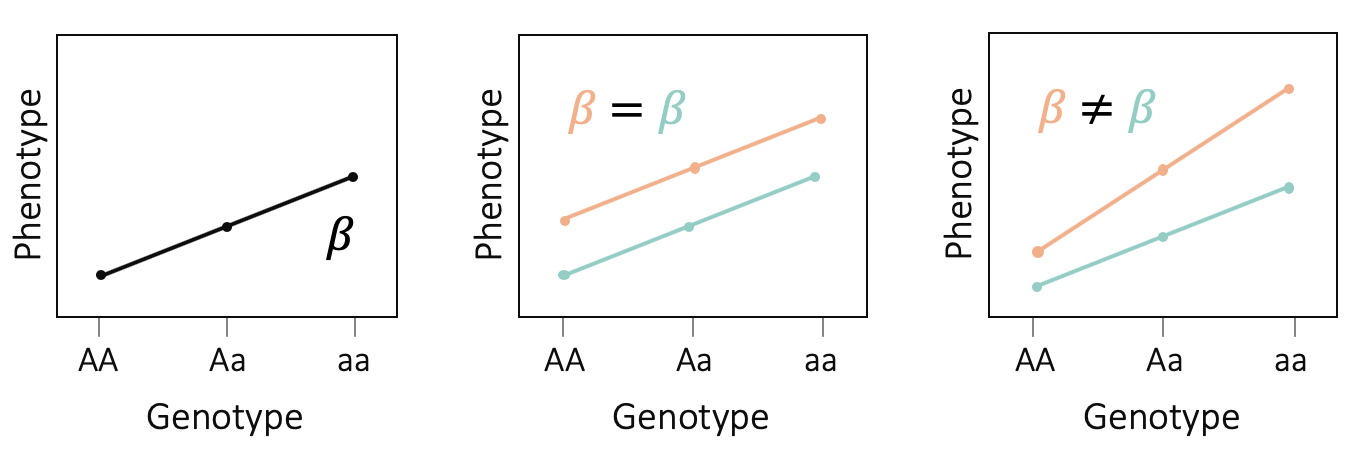
\includegraphics[width=16cm]{Chapter1/Fig/GxE.png}
\caption[Illustration of GxE]{\textbf{Illustration of GxE effect for two environmental groups}.\\
Illustrated are the mean phenotype values across three genotypic groups for a given locus (AA: homozygous major allele, aA: heterozygous individuals, aa: homozygous minor allele).
The first plot (left) describes the case of a genetic effect of the variant on all individuals. 
$\beta$ represents the (in this case positive) effect size of the locus tested. 
The second plot (middle) shows that two groups of individuals characterised by different environmental exposure (represented by the colours). 
The environments have an effect on phenotype (as represented by a shift upwards for the orange group) but the genetic effect remains constant. 
Finally, the third plot (right) shows a GxE effect.
There is an interaction effect between the individuals' genotypes and their environmental exposure, such that for one group (orange) the genetic effect was exacerbated whilst for the other group (seagreen) the effect was dampened.}
\label{fig:gxe}
\end{figure}

% \newpage
In the following, I describe various approaches to test for GxE interactions, which all build on the \gls{lmm} framework. 
% \\
One possible way to detect interaction effects is to stratify samples into discrete subgroups based on their environmental exposure. 
% \\
In \gls{eqtl} mapping, one might for example cluster cells into cell types, or separate samples into different condition groups.
Then, an LM (eq. \eqref{eq:Linear_regression_genetics_covariates}) or \gls{lmm} (eq. \eqref{eq:Linear_mixed_model}) can be applied to each stratum and the marginal variant effects can be compared to assess whether there is a significant difference in these effects across the sub-populations.
This method can be defined as a `stratified interaction test'.
However, as more detailed environmental data is collected, allowing for finer stratification of the population, these methods are no longer optimal as the sub-populations become too small to obtain stable estimates of the variant effects.
For example, as more and more rare cell types are identified and as the definition of cell types becomes more blurred, joint analyses may be preferable. \\

% add reference to multi-tissue eqtl mapping methods

% \subsection{Single environment interaction test}

Another commonly-used method to test for interaction effects is an extension of the LM or \gls{lmm} to include two additional FE terms, an interaction term (GxE) and an environment term (E):

\begin{equation}\label{eq:Interaction_test_FE_LMM}
 \mathbf{y} =  \mathbf{W}\boldsymbol{\alpha} + \mathbf{e}\gamma  + \mathbf{g}\beta_G + \mathbf{e}\odot\mathbf{g}\beta_{GxE} + \mathbf{u} + \boldsymbol{\psi}, 
\end{equation}

where $\mathbf{e}$ represent the environment term, $\gamma$ is its corresponding weight and where two genetic effect terms are present, $\beta_G$ which is the `persistent' genetic effect size whilst $\beta_{GxE}$ is the effect of the interaction term (GxE).
Finally, $\odot$ denotes element-wise multiplication (Hadamard product).
The test is:

\begin{equation}
 H_{0}: \beta_{GxE}=0 
\end{equation}
vs
\begin{equation}
 H_{1}: \beta_{GxE} \neq 0. 
\end{equation}

This model allows to directly test for a GxE interaction effect with a certain environment/factor\footnote{Or with another genetic variant, to test for epistasis \cite{wei2014detecting}.}, beyond the additive effects of the \gls{snp}s and the environment themselves. 
Of course, the same model can also be extended to the case of multi-environment interaction by simply adding more environments as FE terms:

\begin{equation}\label{eq:multi_interaction_test_FE_LMM}
 \mathbf{y} =  \mathbf{W}\boldsymbol{\alpha} + \mathbf{e}_1\gamma_1 + \mathbf{e}_2\gamma_2 + ...  + \mathbf{g}\beta_G + \mathbf{e_1}\odot\mathbf{g}\beta_{GxE,1}+ \mathbf{e_2}\odot\mathbf{g}\beta_{GxE,2} + .. + \mathbf{u} + \boldsymbol{\psi}. 
\end{equation}

However, this becomes quickly infeasible for large numbers of environments, especially for relatively small sample sizes, because of the degrees of freedom loss when increasing the number of parameters to estimate (two additonal parameters to estimate for every environment included). \\

Finally, in the specific context of measuring genetic effects on gene expression, and testing for interactions between environmental exposures and such genetic effects, an alternative approach is to model the effect that these environments have on allele-specific expression (ASE, see \textbf{Box \ref{box:ase}} in the next chapter).
I describe this approach in more detail upon its application in \textbf{Chapter 4} (\textbf{section \ref{sec:endodiff_dynamic_eqtl}}).


% \subsection{StructLMM}
% \label{sec:struct_lmm}

% A recently proposed method called StructLMM (structured linear mixed model) allows for the joint analysis of GxE effect of hundreds of environmental variables \cite{moore2019linear} in an efficient manner.
% In Chapter 6, I will present an extension to StructLMM for applications to scRNA-seq data so I refer the reader to that chapter for derivations of the updated model.
% Instead, I will use this section to give an intuition for the method.\\

% The \gls{lmm} in eq. \eqref{eq:Linear_mixed_model} models the weight of a given \gls{snp} (or effect size, $\beta$) as a scalar, where the assumption is that the effect of a \gls{snp} on the trait is the same across all samples.
% However, as we have seen, samples belonging to different environmental subgroups can have different effects of a \gls{snp} on a trait due to \gls{gxe} effects (\textbf{Fig. \ref{fig:gxe}}).
% Moreover, the sub-grouping might be extremely complex, possibly driven by several environmental exposures, making the addition of them all in the model described in eq. \eqref{eq:multi_interaction_test_FE_LMM} infeasible.

% The intuition of Struct\gls{lmm} is to again consider the \gls{snp} effect size as split into two components, the persistent effect size, which is assumed to be persistent across conditions (we call this $\beta_G$) and the GxE effect size. 
% However, here the GxE effect size is modelled as a random variable and is an $N \times 1$ vector ($\boldsymbol{\beta}_{GxE}$), which depends on the environmental structure of the samples:

% \begin{equation}\label{eq:StructLMM-int}
%  \mathbf{y} =  \mathbf{W}\boldsymbol{\alpha} + \mathbf{g}\beta_G + \mathbf{g} \odot \boldsymbol{\beta_{GxE}} + \mathbf{e} + \boldsymbol{\psi}, 
% \end{equation}

% where $\odot$ denotes Hadamard product, such that $\mathbf{g} \odot \boldsymbol{\beta_{GxE}} = diag(\mathbf{g})\boldsymbol{\beta_{GxE}}$ where $diag(\mathbf{g})$ is an $N \times N$ diagonal matrix, i.e. all off-diagonal elements are 0, diagonal elements correspond to elements of the $N \times 1$ vector $\mathbf{g}$, whereas $\boldsymbol{\beta_{GxE}}$ is a $N \times 1$ vector such that:

% \begin{equation}\label{eq:StructLMM-int_beta_GxE}
%     \boldsymbol{\beta_{GxE}} \sim \mathcal{N}(\mathbf{0}, \sigma^2_{GxE}\mathbf{E}\mathbf{E}^T).
% \end{equation}

% Further, $\mathbf{e} \sim \mathcal{N}(\mathbf{0}, \sigma^2_{e}\mathbf{E}\mathbf{E}^T)$ and $\boldsymbol{\psi} \sim \mathcal{N}(\mathbf{0}, \sigma^2_{n}\mathbf{I})$. 
% The test then is:

% \begin{equation}\label{eq:StructLMM-int_H0}
%  H_{0}: \sigma^2_{GxE}=0 
% \end{equation}
% vs
% \begin{equation}\label{eq:StructLMM-int_H1}
%  H_{1}: \sigma^2_{GxE} \neq 0. 
% \end{equation}

% StructLMM also allows for testing for associations, whilst accounting for GxE effects, essentially testing for any effects of a given variant, either G or GxE.
% However, this is beyond the scope of this thesis so I refer the reader to the original paper \cite{moore2019linear}.\\

% The main limitation of StructLMM is that, for reasons of inference efficiency, it does not properly account for population sub-structure.
% Note that the term $\mathbf{e}$ in \eqref{eq:StructLMM-int} accounts for effects that the environmental sub-structure of individuals might have on the phenotype directly (i.e. not mediated by $\mathbf{g}$).
% However, that leaves no room to account for genetic population sub-structure.
% For unrelated individuals, as we discussed in \textbf{section \ref{sec:pop_struct_noLMM}}, it may be sufficient to include \glspl{pc} as covariates.
% In the case of repeated samples, however, whether it is single cells from the same donor or longitudinal measures from the same individual, that is no longer the case.
% In Chapter 6, I propose a solution for this problem and 
% show preliminary results on a \gls{scrnaseq} dataset.
% % apply the model on a variety of simulated and real \gls{scrnaseq} datasets.

\newpage

\section{Discussion}

Linear mixed models are widely applied in genetic association analysis because they offer great control for confounding effects.
Throughout this thesis, I will use different models for \gls{eqtl} mapping using single cell expression profiles, which all build on this framework.
I have used this chapter to lay the foundation and notation for which we build extensions in the coming chapters.\\

Specifically, in \textbf{Chapter \ref{chapter3}}, I provide a best-practice pipeline for performing bulk-like \gls{eqtl} mapping using single cell data, where I test various aggregation methods as well as design matrices and then use the standard linear mixed model from eq. \eqref{eq:Linear_mixed_model} to map \glspl{eqtl}.
I compare our results to an \gls{eqtl} map obtained using bulk RNA-seq from the same samples and also compare results across scRNA-seq technologies for a subset of donors.
Next, in \textbf{Chapters \ref{chapter4}} and \textbf{\ref{chapter5}} I use different adaptations of linear and linear mixed models to test both for associations (eq. \eqref{eq:Linear_mixed_model}) and interactions (eq. \eqref{eq:Interaction_test_FE_LMM}) in two separate population-scale human \gls{scrnaseq} datasets. 

% Finally, in \textbf{Chapter 
% % 6
% \ref{chapter6}} I present scStruct-LMM, an extension to the StructLMM model (i.e. eq. \eqref{eq:StructLMM-int}) that is able to handle repeated observations from the same samples.
% The model is originally intended for single cell data, and allows to test for context-specific \gls{eqtl} mapping across cell contexts and states.
% However, it could also be used for performing GxE interactions across many variables in any other study with replicated measurements for the same individual, such as longitudinal studies.